\chapter{深度学习，真的行}

%1  什么是深度学习。
%1.1  从机器学习到深度学习 
%1.2. 深度学习的发展史：
%	1.2.1单个神经元 、
%       1.2.2 M-P模型 
%	1.2.3 感知机
%	1.2.4人工神经网路：从简单到深度、多层感知机网络 
%1.3万能逼近定理；
%1.4. 激活函数
%1.5. 没有免费的午餐定理 6.
%
%2.深度学习的组成部分
%
%3.常见的深度学习模型
%   3.1 卷积神经网络
%   3.2 循环神经网络

深度学习，简单来说，就是让计算机变得更聪明的一种方式。它的核心是一个“更深”的神经网络——层数多得像一个会自己思考的“洋葱”，一层包一层，直到揭示数据的真相。

那么，这个“深”的网络是怎么来的呢？它模仿了人类大脑的构造和功能，用数学的方法重现了神经元之间传递信号的机制。说白了，深度学习就是试图让机器拥有一点点“脑子”，尽可能靠近生物神经网络的聪明才智。

想想看，人类是怎么变聪明的？无非是观察世界、提炼规律、然后找到解决问题的方法。深度学习正是想让机器走上这条“智能之路”，从大量数据中学习规律，再把这些规律用到现实中去，比如看图识猫、帮你推荐下一首最喜欢的歌，甚至陪你打《英雄联盟》。听起来是不是很厉害？



深度学习作为机器学习的一个重要分支，在近年来展现了极高的应用价值。从语音识别到图像分类，从自然语言处理到自动驾驶，深度学习以其卓越的表现推动了人工智能的飞速发展。其成功背后依赖于大规模数据、高性能计算以及深层神经网络模型的强大学习能力。

深度学习的核心思想正是从神经科学的研究成果中汲取灵感，通过模拟神经元的行为和结构，逐步构建了强大的人工智能系统。

在本节中，我们将从深度学习的生物学启发出发，逐步介绍单个神经元模型、感知机及其扩展到多层的人工神经网络，探讨深度学习从理论到实践的关键构成。

\begin{figure}[htbp]
\centering
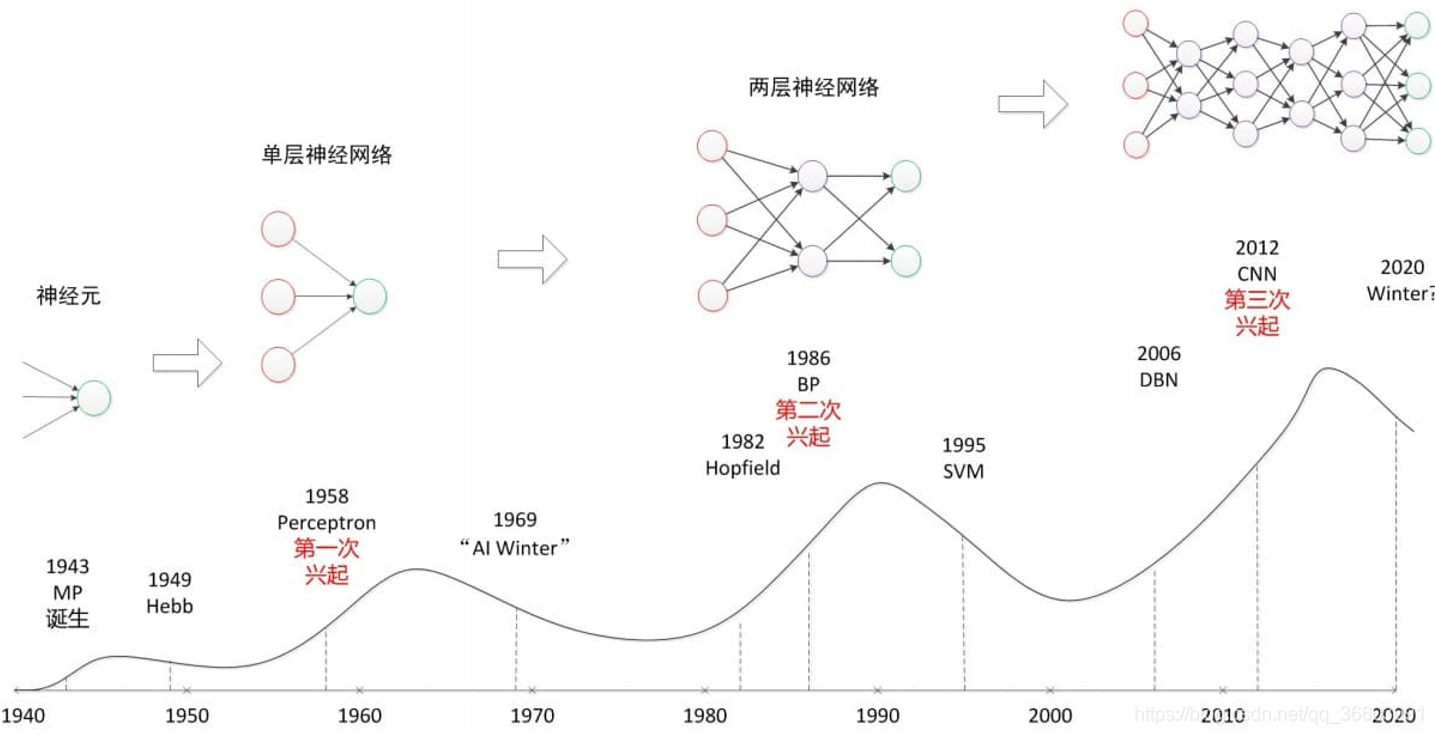
\includegraphics[width=1\textwidth]{figs/ANN.png}
\caption{人工神经网络发展史}
\label{ANN}
\end{figure}


深度学习与强化学习：机器学习的新纪元
深度学习的出现
深度学习通过多层神经网络对数据进行复杂特征的分层提取，显著提高了模型对高维复杂数据的处理能力。

它使得无监督学习在特征学习和生成建模中获得了新的突破。
它在监督学习中实现了端到端的训练，大幅提升了传统任务的性能。
强化学习的崛起
强化学习通过试探和反馈，解决了传统学习方法无法应对的动态决策问题，例如游戏 AI（AlphaGo）、自动驾驶和机器人控制。

机器学习的新范式
深度学习和强化学习的结合，使得机器学习从“标注依赖的模型”转变为“主动学习的智能体”，能够像生物大脑一样从环境中自我学习并适应。


\section{什么是深度学习？}

如第~\ref{ch:机器学习}章中所述， 经典机器学习，通常是用人类的先验知识，把原始数据预处理成各种特征（Feature），然后对特征进行分类。然而，这种分类的效果，高度取决于特征选取的好坏。传统的机器学习专家们，把大部分时间都花在如何寻找更加合适的特征上。因此，早期的机器学习专家非常辛苦。传统的机器学习，其实可以有一个更合适的称呼—特征工程（Feature Engineering）。

后来，机器学习的专家们发现，可以让神经网络自己学习如何抓取数据的特征，这种学习方式的效果似乎更佳。于是兴起了特征表示学习（Feature Representation Learning）的风潮。这种学习方式，对数据的拟合也更加灵活好用。于是，人们终于从自寻特征的痛苦生活中解脱了出来。

但这种解脱也需要付出代价，那就是机器自己学习出来的特征，它们存在于机器空间，完全超越了人类理解的范畴，对人而言，这就是一个黑盒世界。为了让神经网络的学习性能表现得更好，人们只能依据经验，不断尝试性地进行大量重复的网络参数调整，同样是苦不堪言。于是，人工智能领域就有了这样的调侃：“有多少人工，就有多少智能”。

因此，你可以看到，在这个世界上，存在着一个“麻烦守恒定律”：“麻烦不会减少，只会转移。”

再后来，网络进一步加深，出现了多层次的“表示学习”，它把学习的性能提升到另一个高度。这种学习的层次多了，其实也就是套路深了。于是，人们就给它取了一个特别的名称—Deep Learning（深度学习）。

简单来说，深度学习就是一种包括多个隐含层（越多即为越深）的多层感知机。它通过组合低层特征，形成更为抽象的高层表示，用以描述被识别对象的高级属性类别或特征。能自生成数据的中间表示（虽然这个表示并不能被人类理解），是深度学习区别于其他机器学习算法的独门绝技。

\section{从机器学习到深度学习}
机器学习的核心任务是从数据中学习模式，而深度学习则是机器学习的一个子领域。其主要特点是利用多层神经网络自动从数据中提取特征，从而省去了传统机器学习中繁琐的特征工程步骤。
深度学习的最大突破在于其层级式特征表示的能力——从浅层特征（如图像中的边缘）逐步学习到深层语义特征（如图片中的物体类别）。这一特性使深度学习在处理高维复杂数据时具有独特的优势。


{\bf 深度学习和机器学习的区别}

以模式分类为例，在传统的机器学习把特征提取和分类处理为两个独立的步骤，整个学习流程，需要人为的划分子问题。而以CNN为代表的深度学习，则为我们提供了另一种范式（paradigm），即“端到端（end-to-end）”学习方式，它把特征提取和分类任务合二为一，完全交给深度学习模型，直接学习从原始输入到期望输出的映射。如下图所示。
\begin{figure}[htbp]
\centering
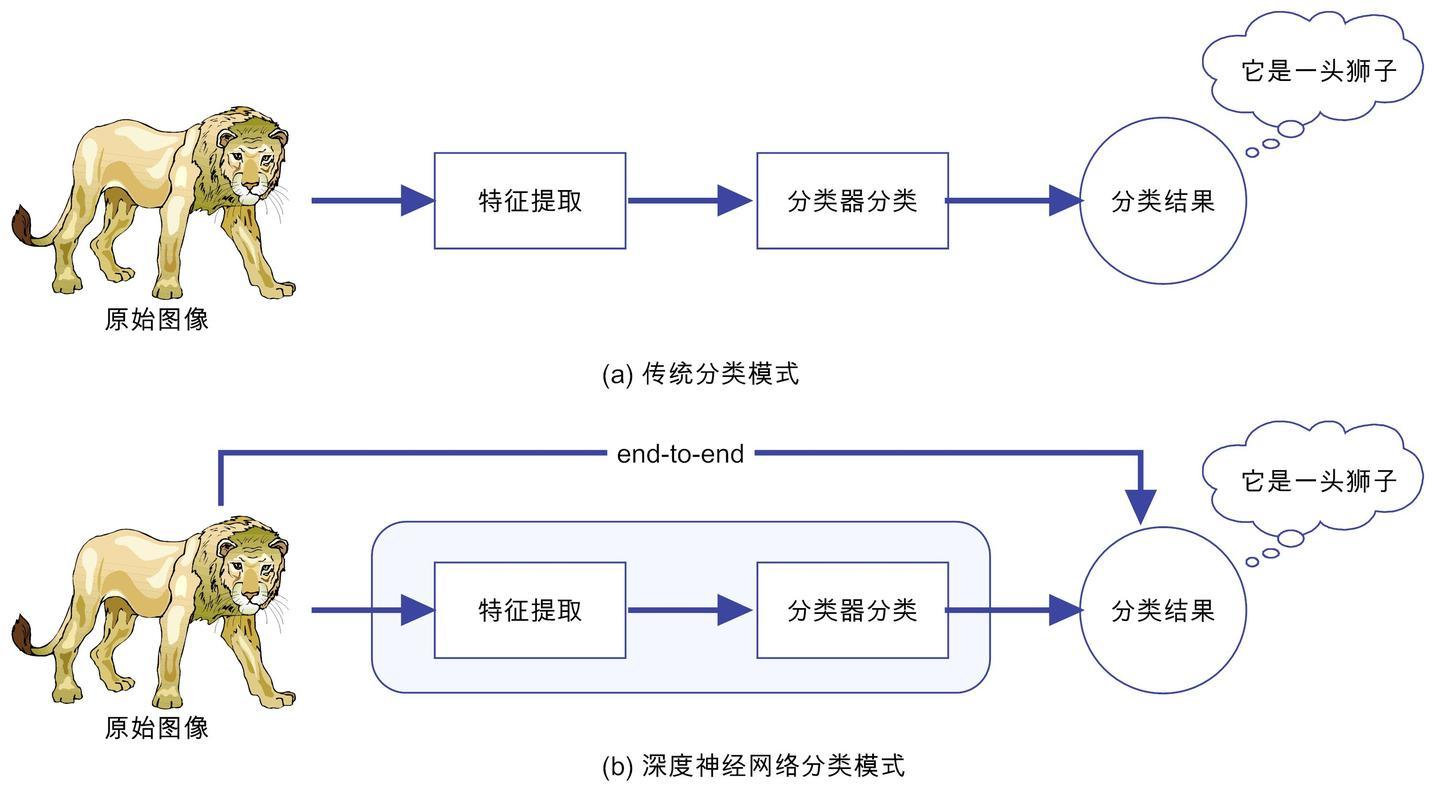
\includegraphics[width=1\textwidth]{figs/传统模式分类与深度神经网络的区别与联系.jpg}
\caption{传统模式分类与深度神经网络的区别与联系}
\label{ANN}
\end{figure}

这里“end-to-end”（端到端）说的是，输入的是原始数据（始端），然后输出的直接就是最终目标（末端）。整个学习流程并不进行人为的子问题划分，而是完全交给深度学习模型直接学习从原始输入到期望输出的映射。


%\subsection{ 一波三折的联结学派}
\section{深度学习：智能的层层递进}
深度学习，顾名思义，“深度”学习。

深度学习的故事始于对生物神经元的模仿，从神经元的启发，到简单的数学模型，再到多层神经网络的奇妙构造，这场革命性的旅程为人工智能开辟了全新的方向。

深度神经网络的本质是层数较多的神经网络。它模仿生物神经网络的行为特征，试图通过分布式并行处理实现对复杂问题的求解。那么，什么是神经网络？简单来说，它是一个算法模型，通过对输入数据的逐层处理，最终实现对问题的解决。

人类天生具有智能，这种能力来源于大脑复杂的神经网络。如果想让“人造物”具备类似的智能，模仿人类无疑是最自然的选择。早在春秋时期，老子在《道德经》中提出“人法地，地法天，天法道，道法自然”，这句古老的哲思正隐含了深度学习的启示：效法自然，寻求智慧。

比如，雷达的发明来源于对蝙蝠声呐导航的研究，潜水艇的构想则受启于鱼鳔的功能。同样，人们也希望通过研究人类大脑神经网络的工作原理，找到实现人工智能的方法。人工神经网络（Artificial Neural Network，ANN）正是在这种探索中应运而生。
深度神经网络，就是比较“深”的神经网络，即层数较多的神经网络。

那什么是神经网络呢？简单来说，它是一种模仿动物神经网络行为特征，进行分布式并行处理信息的算法模型。

人，无疑是有智能的。如果想让“人造物”具备智能，模仿人类是最朴素不过的方法论了。早在春秋时期，老子便在《道德经》中给出了自己的睿智判断：
“人法地，地法天，天法道，道法自然。”
这里所谓的“法”，作为动词，为“效法、模仿、学习”之意。特别是“道法自然”的含义，意味悠长。的确，大道运化天地万物，无不是遵循自然法则的规律。人们从“自然”中学习和寻求规律，在很多时候，的确比自己苦思冥想更加可行和高效。

比如，人们从研究蝙蝠中获得发明雷达的灵感，从研究鱼鳔中获得发明潜水艇的启迪。很自然的，人们同样期望研究生物的大脑神经网络，然后效仿之，从而获得智能。

人工神经网络（Artificial Neural Network，ANN）便是其中的研究成果之一。


\subsection{生物神经元的启发}

人，无疑是有智能的。如果想让“人造物”具备智能，模仿人类是最朴素不过的方法论了。早在春秋时期，老子便在《道德经》中给出了自己的睿智判断：

“人法地，地法天，天法道，道法自然。”

这里所谓的“法”，作为动词，为“效法、模仿、学习”之意。特别是“道法自然”的含义，意味悠长。的确，大道运化天地万物，无不是遵循自然法则的规律。人们从“自然”中学习和寻求规律，在很多时候，的确比自己苦思冥想更加可行和高效。

这句老子的话，用在深度学习的起源上，似乎再合适不过了。既然人类本身就是智能的，那为什么不向人类自身学习呢？于是，科学家们将目光投向了大脑。

比如，人们从研究蝙蝠中获得发明雷达的灵感，从研究鱼鳔中获得发明潜水艇的启迪。很自然的，人们同样期望研究生物的大脑神经网络，然后效仿之，从而获得智能。

人工神经网络（Artificial Neural Network，ANN）便是其中的研究成果之一。

大脑作为人类认知的中心，其工作机制复杂而神秘，但底层逻辑却可能源于神经元简单而有效的信号传递模式。

通过研究神经元的信号传递机制，科学史上，我们第一次知道了“我们是怎么知道的”！

大脑的工作机制复杂而神秘，但其底层逻辑，是不是也构建于神经元的简单输出？

比如，神经元的“兴奋与抑制”机制被认为是一种自然的开关，可以类比成数字电路中的逻辑门。科学家发现，大脑通过简单规则叠加出复杂功能的能力，为人工神经网络的设计提供了重要的启发。

神经元的激活模式为人工神经网络的构建提供了直接的参考。简单的加权求和和非线性激活的数学模型能够捕捉复杂的模式，使得人工智能具备了模拟大脑的基础能力。

认知神经科学从弗洛伊德的定性精神分析走向了计算神经学，将认知神经学和脑科学从玄学的边缘挽救回来，成为了一门真正的科学。

神经元是生物学启发的起点。早在 20 世纪初，科学家发现神经元通过电信号相互连接并传递信息。每个神经元的作用是接收输入信号，经过处理后输出一个信号给其他神经元。

深度学习的灵感最早来源于对生物神经系统的模拟。人类大脑有约 $10^{11}$ 个神经元，通过$10^{14}$ 个突触连接形成庞大的网络。虽然单个神经元只会简单地接收、处理和传递信号，但当成千上万个神经元“抱团”工作时，它们就能完成从感知到思考的复杂任务，其处理信息的效率和能力远远超出现有计算机系统。这种自然的并行计算机制为人工神经网络的设计提供了重要启示。

人类对神经系统的认识始于 19 世纪末的神经元学说。Cajal 的研究首次揭示了神经元作为神经系统基本单位的独立性，为后来的神经科学研究奠定了基础。此后，神经元传递信号的方式被逐步揭示，为人工神经网络的构建提供了理论依据。

生物神经元的基本结构包括三个部分：
1. 细胞体（Soma）： 负责接收和整合来自其他神经元的信号，判断是否发出信号。
2. 树突（Dendrite）： 接收其他神经元通过突触传递来的输入信号。
3. 轴突（Axon）： 将整合后的信号传递给下一个神经元。

{\bf 神经元的工作机制}
生物神经元通过电信号和化学信号进行通信。
在静息状态下，神经元处于抑制状态，不会主动传递信号。树突接收输入信号后，信号在细胞体中进行累积，当累积信号超过一定阈值时，神经元会被激活，并通过轴突将信号传递给其他神经元。这些信号刺激下游神经元，从而在神经网络中传播。这一过程中的关键机制包括信号加权、累积和激活。

这种简单而高效的机制被认为是大脑复杂信息处理能力的基础。正如麦克洛克和皮兹在 1943 年提出的假设，大脑的复杂功能可能建立在神经元简单行为的重复和组合之上。这一假设不仅激发了认知科学的研究热潮，也成为人工神经网络设计的灵感来源。

ANN的性能好坏，高度依赖神经系统的复杂程度，它通过调整内部大量“简单单元”之间的互连权重，从而达到处理信息的目的，并具有自学习和自适应的能力。这里的的“简单单元”，就是神经网络中的最基本元素—神经元（Neuron）模型。在生物神经网络中，每个神经元与其他神经元通过突触进行连接。神经元之间的信息传递，属于化学物质的传递。当它“兴奋”时，就会向与它相连的神经元发送化学物质（神经递质，Neurotransmitter），从而改变这些神经元的电位。如果某些神经元的电位超过了一个阈值，那么，它就会被“激活”，也就是“兴奋”起来，接着向其他神经元发送化学物质，犹如涟漪，就这样一层接着一层传播，如图~\ref{大脑神经细胞的工作流程}所示。
\begin{figure}[htbp]
\centering
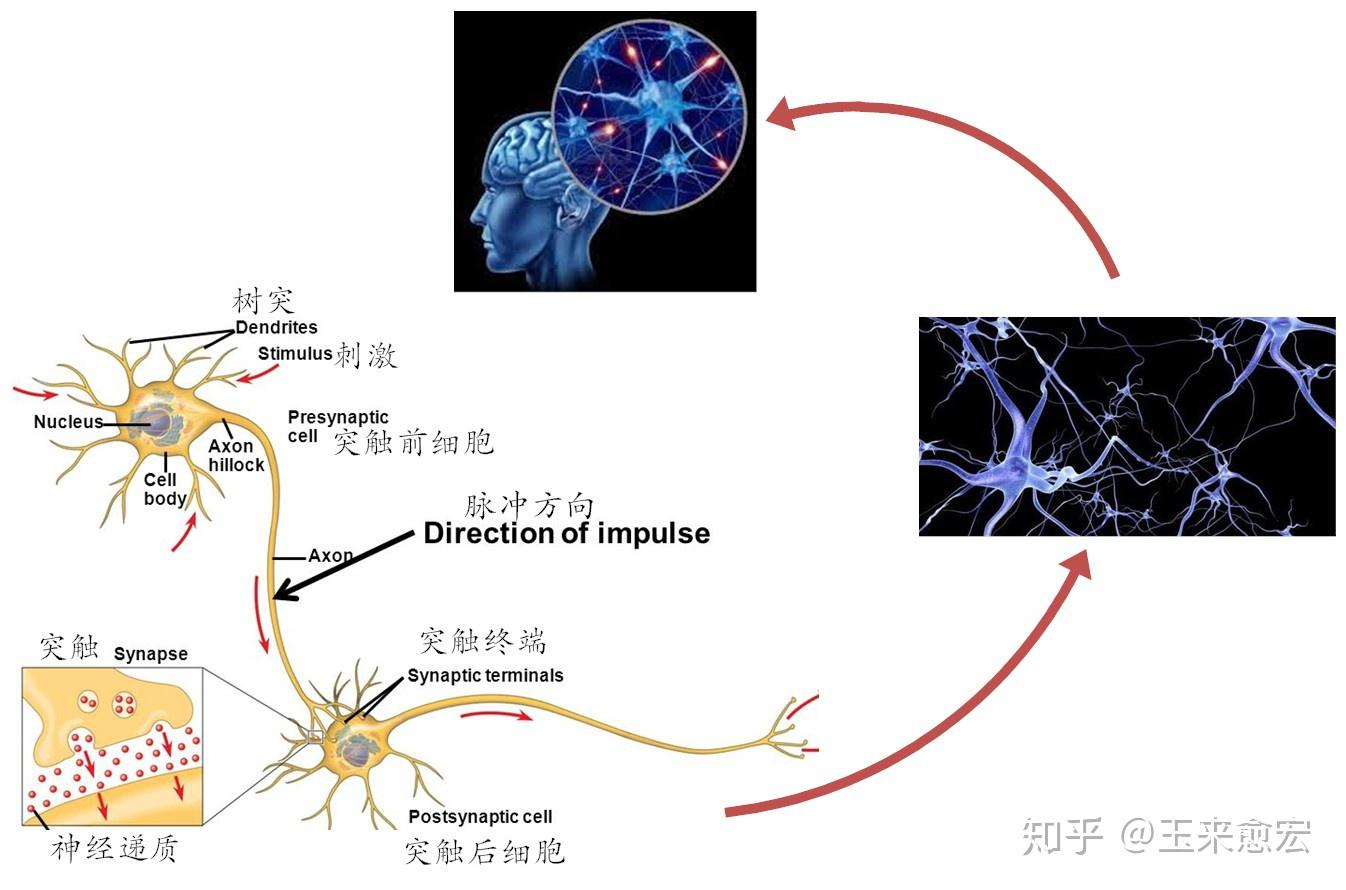
\includegraphics[width=1\textwidth]{figs/大脑神经细胞的工作流程.jpg}
\caption{大脑神经细胞的工作流程}
\label{大脑神经细胞的工作流程}
\end{figure}

\subsection{M-P模型：神经网络的起点 }

模仿大脑神经元的最早示例，就是20世纪40年代提出但一直沿用至今的“M-P神经元模型”。

M-P神经元模型最早源于发表于1943年的一篇开创性论文。论文的两位作者分别是神经生理学家沃伦·麦克洛克（Warren McCulloch）和数学家沃尔特·皮茨（Walter Pitts），他们用一个简单的数学模型模拟神经元的行为？他们提出了被称为“M-P模型”的神经元计算模型，成功将神经科学和数学逻辑结合在了一起。

这个模型是怎么回事？简单来说，M-P模型像是一个“简单的电路”。它接收多个输入信号（比如神经元的树突接收外界刺激），把这些信号加权求和（模拟信号的强弱），再通过一个激活函数判断是否“触发”输出。如果信号总和超过某个阈值，神经元就“兴奋”了；否则，它就保持“沉默”。

看起来很简单对吧？但这却是人工神经网络的起点。麦克洛克和皮茨的论文后来被誉为“神经网络天下第一文”，不仅为人工智能打下了理论基础，还在很大程度上催生了现代计算机科学的发展。


首次实现了用一个简单电路（即感知机）来模拟大脑神经元的行为。
皮茨等人的研究，据说甚至影响了控制论的诞生和冯·诺伊曼计算机的设计。

麦克洛克比皮茨大一辈，皮茨1923年刚出生，麦克洛克已经年方25。与皮茨相比，麦克洛克的世界可谓有泥云之别。
麦克洛克出生于美国东岸的一个优越家庭，中学就读新泽西州贵族男校，本科在耶鲁大学学习哲学和心理学，之后又在哥伦比亚大学取得了心理学硕士和医学博士。这一路走来，升级打怪，顺风顺水。

后来，麦克洛克毕业后做了几年实习医生，先去了耶鲁大学研究神经生理学，之后又去了伊利诺伊大学芝加哥分校，做精神病学系的教授。

皮茨（18岁）遇见麦克洛克时，42岁的麦克洛克正值盛年，他已是一位受人尊敬的科学家。麦克洛克的学术生涯铸就了他具备一个杂家的潜质。但在内心深处，麦克洛克却向往成为一名哲学家，他就想弄明白，知识的终极意义是什么。

1923年（也就是皮茨出生的那年），如日中天的心理学大师弗洛伊德（Freud）出版了著作《自我与本我》（The Ego and the Id），精神分析热潮迭起。但是，麦克洛克对此却不以为然。他坚持认为，精神世界中的神秘工作及精神的失常，不过来源于大脑神经元的正常或失常反应而已，而这是纯机械式的。

麦克洛克的强项是神经科学，但他不擅长数学，难以形式化描述自己的思维。而颇有数学才华的皮茨，正好可以补其短板。

受《数学原理》的启发，麦克洛克当时正尝试做一件极富挑战性的事，即用戈特弗里德·莱布尼茨（Gottfried Leibniz，1646—1716，哲学家、数学家、微积分和二进制的发明人）的逻辑演算，来构建一个大脑模型。

罗素等人在书中论述说，“所有的数学法则，都可自下而上地用无可辩驳的基本逻辑来建立（all of mathematics could be built from the ground up using basic, indisputable logic）”。而在底层、基础的逻辑，即为是与非两种判定。然后，通过对这两个逻辑判定进行一系列的组合操作，例如，合取（conjunction）实现“与（and）”操作、析取（disjunction）实现“或（or）”操作、取反（negation）实现“否（not）”操作，这样就可以一砖一瓦地构建起复杂的数学大厦。

罗素等人的论断，在思想上，其实算不上创新。早在春秋时期，老子就在《道德经》写下了明断，“道生一，一生二，二生三，三生万物”。无论是罗素等人的论断，还是老子的明断，在哲学上，都同属还原论（Reductionism）的范畴。

比如，在古代，前人的智慧，描述得并不十分清晰，如果你想得“道”，就得自己去“悟”前人的成果。而这个“悟”，其程度通常因人而异，如果“悟”得五花八门，那前人的智慧就会被拆分得“七零八落”，因此，前人的学问就非常容易陷入“玄学”之列。一旦知识的继承性成了问题，那么知识的积累也就成了问题。而如果没有了知识的积累，就很难引爆知识的“质变”。

相比而言，西方社会从欧几里得的《几何原本》开始，不论是莱布尼茨的“二进制”，还是罗素等人关于数学的论断，它们都有一套清晰可见的规则，可供人们任意复盘公理化推演。

如此一来，知识的可重复性（或者说可继承性）就非常高。当西方基于精确性思维的知识，积累到一定程度后，很容易发生知识的“质变”。发生在14世纪到16世纪的文艺复兴（Renaissance），就是这一质变的结果。

当下进入了“数据技术（DT）”时代，在这个时代，不论东方还是西方，人们对可重现数据的重视，都达到无以复加的地步，从而也拉动了人们从数据中寻找智慧（即人工智能）的步伐。中国在人工智能领域，扮演着愈发重要的角色。

{\bf 神经元工作机理之初探}

医学知识告诉他，大脑中的每一个神经元细胞，只有当外部刺激超过最小阈值时，才被激发，否则就处于静默状态。这些外部刺激，来自与之相邻的神经元，它们通过突触来传递信号。从人的反应消耗能量来看，这一设置非常智能。 ...

神经元细胞的二元工作状态（即激发或静默），让麦克洛克联想到了莱布尼茨二进制逻辑单元以及罗素的数学构建论断。大脑的工作机制复杂而神秘，但其底层逻辑，是不是也构建于神经元的简单输出呢？



于是，麦克洛克猜想，{\bf 神经元的工作机制很可能类似于逻辑门电路，它接受多个输入，然后产生单一的输出。通过改变神经元的激发阈值以及神经元之间的连接程度，就可以让它执行“与”“或”“非”等功能。}

当时，麦克洛克刚读了一篇英国数学家阿兰·图灵（Alan Turing）的论文。在论文中，图灵在理论上证明了建造一种可在有限步骤里完成任何计算功能的机器的可能性。这种机器被后人称为“图灵机（Turing Machine）”，它是现代计算机的原型，如图~\ref{图灵机}所示。
\begin{figure}[htbp]
\centering
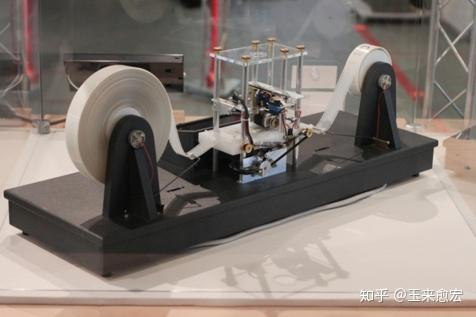
\includegraphics[width=1\textwidth]{figs/图灵机.jpg}
\caption{图灵机}
\label{图灵机}
\end{figure}

所谓的图灵机，是指一台抽象的机器，它采用一条无限长的纸带作为临时存储。纸带分成若干个小方格单元，每个方格单元代表某个符号。它还有一个可读可写的机器头（read-write head，相当于现代意义上的CPU），在纸带上左右移动。机器头有一组内部状态或一些固定的程序。在每个时刻，机器头都要从当前纸带上读入一个方格信息，然后结合自己的内部状态查找程序表，根据程序输出信息，将信息回写到纸带方格上，并转换自己的内部状态，然后继续移动，重复前面的操作。

麦克洛克认为，大脑的工作机理很可能也是这样的一种机器，它用编码在神经网络里的逻辑来完成计算。如果神经元可用逻辑规则连接起来，这样就构建了结构更为复杂但功能更加强大的思维链（Chains of Thoughts）。这种方式与《数学原理》将简单命题链（Chains of Propositions）连接起来，以塑造更加复杂的数学定理，是一致的。

当麦克洛克向皮茨解释他的创意时，皮茨马上就心领神会，并很清楚解决该问题的数学工具。没有碰到皮茨之前，麦克洛克的研究一直陷入瓶颈状态。在一个阡陌纵横的网状神经元系统中，神经元之间的链接路径很可能形成一个环状，即最后一个神经元的输出，就会成为第一个神经元的输入，这是一个头部追逐尾巴的神经网络。

麦克洛克的数学功底并不扎实，因此没办法构建这样的数学模型。因为从逻辑的角度来看，这个首尾相接的环，就如同一个逻辑悖论：后发生的成了先发生的，“结果”成了“原因”。如果把链条的每个环节都贴上一个时间戳的话，第一个神经元在t时间被激发，下一个神经元就会在t+1时刻被激发，依次传递。但如果链条形成环状，t+n时间后，却又仿佛跑到了t时刻的前面，这是多么奇怪啊。

困扰麦克洛克的逻辑难题并没有难倒皮茨，他使用模数（Modulo Mathematics）方法，通过取模操作，把最后一个输出巧妙地变成了第一个输入。就像时钟（模数为12）刻度那样形成环状的数字，12点的下一个钟点，不是顺理成章的13点，而是最开始的1点。

皮茨向麦克洛克阐明，t+n时刻的输出，跳回t时刻之前变成输入，并非悖论。因为在皮茨的计算里，“在前”或“在后”是没有意义的。进一步来说，在他的算式里，压根就不需要时间。一个“挤掉了时间的观念”，在某种程度上，它就是“记忆”。

读者学到后面的章节就会知道，深度学习还有一个重要的分支——循环神经网络（Recurrent Neural Network，RNN），RNN大致遵循类似的工作机制。谷歌前资深计算机科学家吴军博士把“Recurrent Neural Network”翻译成“复发神经网络”，从“可再现”的角度来看，似乎更加合理。

当麦克洛克和皮茨完成他们的计算实验时，实际上，他们完成了一个操作性非常强的机械论精神模型。后人就用二人名称的首字母称呼这个模型——M-P神经元模型。

{\bf 神经网络天下第一文}

信号在大脑中到底是怎样传输的呢，确切来说，到如今这依然是一个谜。于我们而言，“M-P神经元模型”的重要意义在于，我们可以把大脑视为与计算机一样的存在，神经细胞有两种状态：兴奋和不兴奋（即抑制），可利用数字计算机中的一系列0和1进行模拟。通过把简化的二进制神经元连成链条和链环，他们向世人阐明了，大脑能实现任何可能的逻辑运算，也能完成任何图灵机可以完成的计算。这是何等之酷！

这样一来，神经元的工作形式，就类似于数字电路中的逻辑门，它接受多个输入，然后产生单一的输出。通过改变神经元的激发阈值，就可完成“与”“或”及“非”等三个状态的转换功能，如图~\ref{神经网络天下第一文《神经活动中思想内在性的逻辑演算》中的逻辑门（发表于1943年）}所示。
\begin{figure}[htbp]
\centering
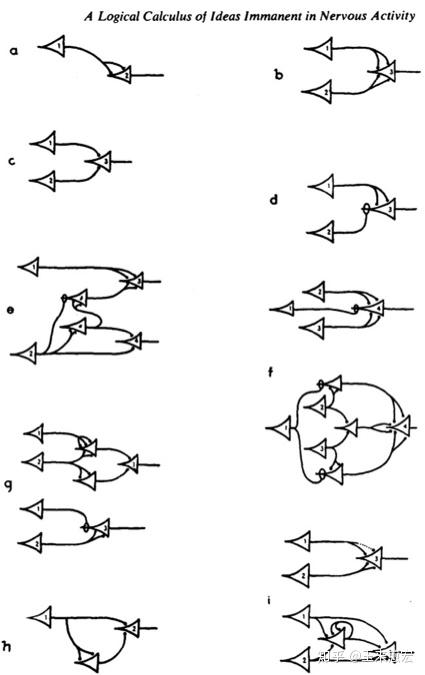
\includegraphics[width=0.6\textwidth]{figs/神经网络天下第一文《神经活动中思想内在性的逻辑演算》中的逻辑门（发表于1943年）.jpg}
\caption{神经网络天下第一文《神经活动中思想内在性的逻辑演算》中的逻辑门（发表于1943年）}
\label{神经网络天下第一文《神经活动中思想内在性的逻辑演算》中的逻辑门（发表于1943年）}
\end{figure}

不同于弗洛伊德的心理学模型，“M-P神经元模型”是第一个将计算用于大脑的应用，同时也衍生出一个著名的论断——本质上，大脑不过就是一个信息处理器。  ---计算神经学

基于他们的研究发现，麦克洛克和皮茨写了一篇学术文章，发表在《数学生物物理学通报》（Bulletin of Mathematical Biophysics）上。这篇文章就是神经网络的天下第一文：《神经活动中思想内在性的逻辑演算》（A Logical Calculus of Ideas Immanent in Nervous Activity）~\cite{mcculloch43a}。这篇文章后来也成为控制论的思想源泉之一。

麦克洛克和皮茨提出的“M-P神经元模型”，是对生物大脑的极度简化，但却成功地给我们提供了基本原理的证明。有了麦克洛克和皮茨等人的研究，在某种程度上，关于“思想”的理解，就变得更加具有可解释性，而不必笼罩一层弗洛伊德式的神秘主义，然后在自我与本我之间牵扯不清。于是，麦克洛克向一群研究哲学的学生骄傲地宣布：
“在科学史上，我们首次知道了我们是怎么知道的（For the first time in the history of science, we know how we know）。”

M-P模型刻画的神经元模型

皮茨在维纳（控制论创始人）的鼓励下，验证M-P模型的功能性，”随着长时间对神经元阙值的调整，这种随机性会渐渐让位于有序性，而信息就涌现出来了。“事实上，上述结论依然适用于现代如火如荼的深度学习。

然后，“调整神经元阙值”这事说起来简单，但做起来可就没有那么简单。当时，对神经元的调整当时还不能自动进行。直到1957年Rosenblatt提出来感知机模型。麦卡洛克和皮茨的神经元模型还可以被描述图~\ref{M-P模型的另一种描述}所示的样子。
\begin{figure}[htbp]
\centering
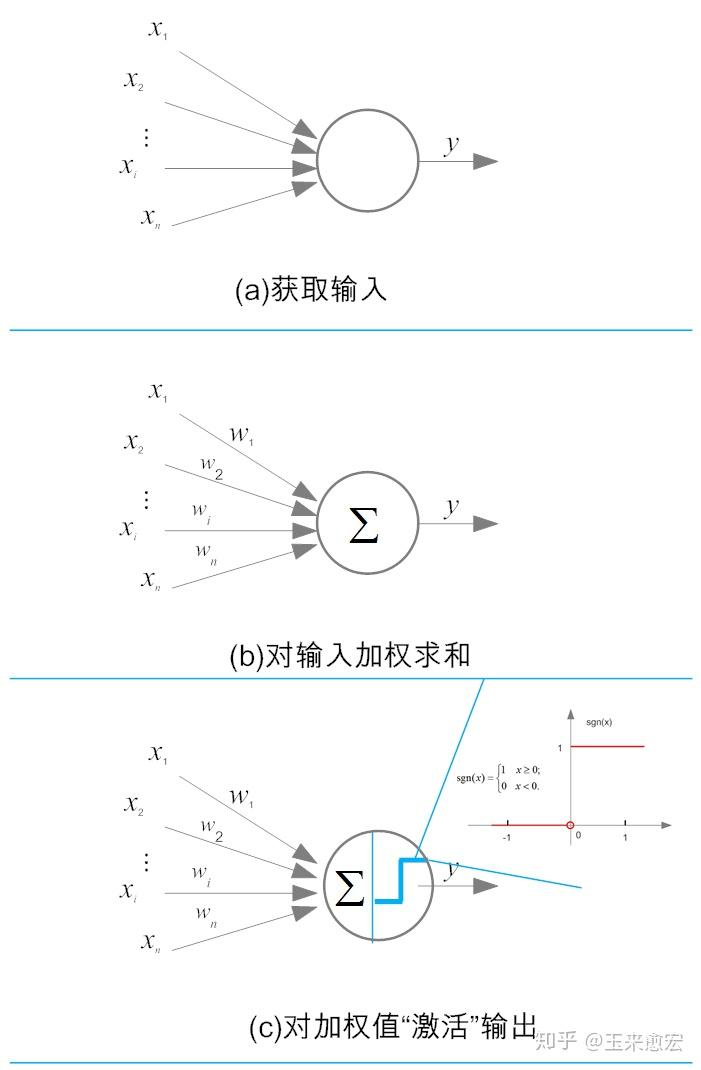
\includegraphics[width=0.8\textwidth]{figs/M-P模型的另一种描述.jpg}
\caption{M-P模型的另一种描述}
\label{M-P模型的另一种描述}
\end{figure}

图~\ref{M-P模型的另一种描述}的描述与现在神经网络中的表示几乎没什么差别了，图~\ref{M-P模型的另一种描述}(a）表示神经元从外界获得输入 ~$x_1,x_2,\dots, x_n$ (箭头模拟表示突触)，传给神经元，神经元的输出是~$y$。图~\ref{M-P模型的另一种描述}(b)突触根据不同的性质以及强度，赋予一个不同的权重，然后，神经元的输入现在升级为一个加权和。图~\ref{M-P模型的另一种描述}(c)表示的是，加权和并不是“赤裸裸”地直接输入，而是阈值函数（亦称激活函数）将“全（1）或无（0）“法则，引入到神经元结构中，这个法则模拟的是神经元激活或抑制。

下面我们对比一下M-P模型和感知机模型的差异。感知机模型如图~\ref{感知机模型}所示。
\begin{figure}[htbp]
\centering
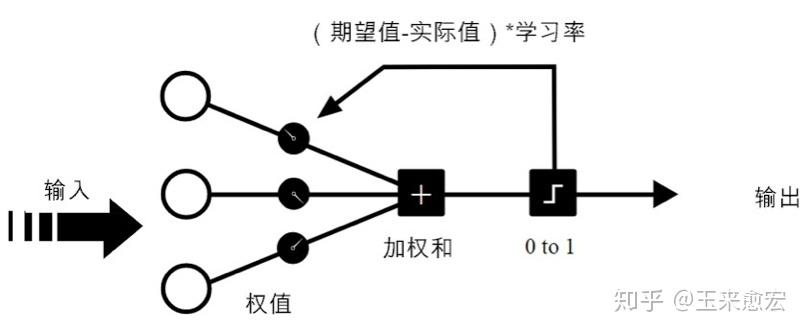
\includegraphics[width=0.8\textwidth]{figs/感知机模型.jpg}
\caption{感知机模型}
\label{感知机模型}
\end{figure}

对比图~\ref{M-P模型的另一种描述}和图~\ref{感知机模型}可知，简单来说，感知机模型就是一个带有反馈机制的神经元。由于感知机模型会在后续的章节中提到，这里不展开。



1943年，神经生理学家麦克洛克和数学家皮兹提出了单个神经元的计算模型—M-P模型，用一个简单电路来模拟大脑神经元的行为。 如图~\ref{生物神经元与人工神经元}所示。
\begin{figure}[htbp]
\centering
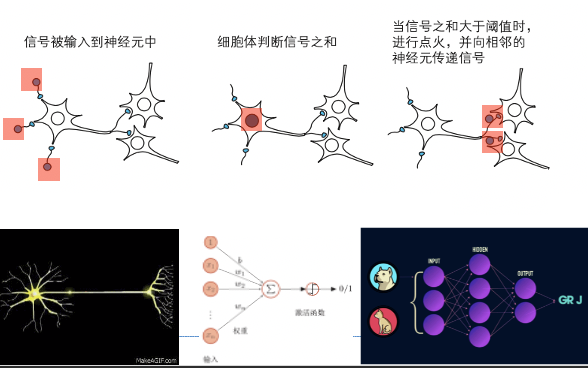
\includegraphics[width=1\textwidth]{figs/neuron.png}
\caption{生物神经元与人工神经元}
\label{生物神经元与人工神经元}
\end{figure}

\begin{figure}[htbp]
\centering
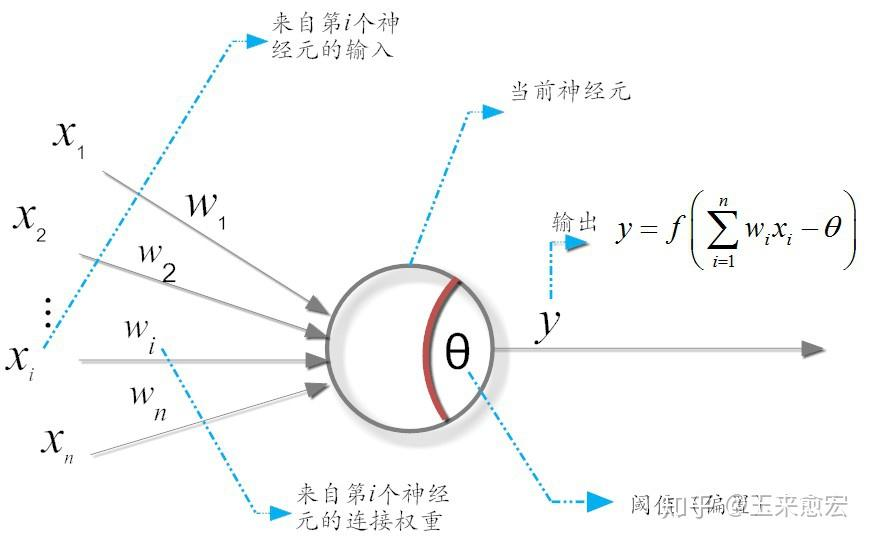
\includegraphics[width=1\textwidth]{figs/M-P神经元模型.jpg}
\caption{M-P神经元模型}
\label{M-P神经元模型}
\end{figure}
M-P 模型通过加权求和和阈值激活机制来模拟神经元的行为。在这个模型中（如图\ref{M-P神经元模型}所示），神经元接收来自n个其它神经元传递过来的输入信号。这些信号的表达，通常通过神经元之间连接的权重（weight）大小来表示，神经元将接收到的输入值按照某种权重叠加起来。叠加起来的刺激强度~$y$可用以下公式表示：
$$
y =\left\{ \begin{array}{ll} 
1 & \mbox{ if } \sum_{i=1}^n w_i x_i\ge \theta\\
0 & \mbox{ if } \sum_{i=1}^n w_i x_i< \theta\\ \end{array}\right.
$$
其中~$x_i$ 表示输入，~$w_i$ 表示权重，~$\theta$ 表示激活阈值，~$y$表示最终的输出(~$0$ 或~$1$)。 
M-P 模型能够实现简单的逻辑运算（如 AND 和 OR），为神经网络研究提供了数学基础。


 M-P模型的价值所在
 
M-P模型的价值至少体现在如下三个方面：
（1）将生理学关于神经系统的研究，带入到数学领域，并与逻辑学相结合。直到现在，很多人还认为，生物学和逻辑学是计算机的未来，为了使机器具有智能，我们必须回归对神经科学或者大脑的研究。

（2）一定程度上，M-P模型催生了现代计算机科学的诞生。在M-P模型中，一方面，现代计算机科学部分借鉴了由神经元构成的神经网络实现的逻辑计算，另一方面，也为存储程序设计带了最原始的参考，M-P模型为图灵机和现代的存储程序计算机之间，搭建了一座难以忽略的桥梁。

（3）M-P模型激发了神经网络学习的发展。一开始，M-P模型神经网络的参数无法实现真正的学习，从皮茨开始，就有一些研究者源源不断的地致力于让神经网络自动学习。于是诸如感知机、BP算法、CNN、RNN、DBN等算法纷纷如雨后春笋般被提了出来，它们都是致力于在不同应用场景下，自动快速找到网络的连接权值。目前，神经网络学习（包括深度学习）已经占据了人工智能领域的半壁江山，M-P模型可谓居功至伟。

当然，M-P模型的成功，还为维纳提出的控制论奠定了一定的基础。

在 Cajal 的神经元学说和麦克洛克、皮兹的数学模型之间，科学史实现了一次重要的飞跃：人类不仅能够观察神经元的行为，还能够用精确的数学语言描述和预测这些行为。这种从定性到定量的转变，不仅挽救了认知神经学和脑科学，使其脱离了玄学的边缘，也为人工智能的崛起提供了坚实的理论框架。
 
M-P 模型被认为是现代人工神经网络的雏形。


牛掰扫地僧：M-P模型背后的那些人和事，参见\cite{张玉宏2018}。

\subsection{感知机(Perceptron)：从神经元到网络，神经网络的“Hello World”}

1957年，Frank Rosenblatt 基于 M-P 模型提出了感知机（Perceptron），这是第一个可以“自学”的神经网络。你可以把感知机看作是神经网络的“Hello World”，它能学会简单的分类任务，比如判断一个水果是“香蕉”还是“西瓜”。

感知机的基本操作很简单：输入一些特征（比如颜色和形状），通过一堆加权计算，再用激活函数输出结果。如果感知机猜错了，它会调整权重，直到能准确分类。这个“试错-调整”的过程，就是机器学习的雏形。

尽管感知机只能解决简单的线性问题，但它的提出点燃了人们对智能机器的期待。《纽约时报》甚至预言：“未来的机器将能识别人类、即时翻译语言，甚至写作诗歌。”虽然当时这些构想有些“天马行空”，但六十年后的今天，这些愿景几乎都已成真。

%---
感知机（Perceptrons），受启发于生物神经元，它是一切神经网络学习的起点。感知机学习，就是神经网络学习的“Hello World”，是很多从事计算机行业的人“光荣与梦想”开始的地方。


“感知机”作为一个专业术语，是皮茨等人发表论文15年之后，即在1958年，由康奈尔大学心理学教授弗兰克•罗森布拉特（Frank Rosenblatt）提出来的。

这位罗森布拉特，说来也是一位奇人，不仅聪慧过人，爱好亦颇为广泛。除了平时酷爱钻研大脑的学习迁移机理之外，他还“折腾”天文学。据说罗森布拉特的一天通常是这样度过的：白天在实验室解剖解剖蝙蝠，研究一番动物大脑的学习机制，夜晚则在自家的后山上，搭建一所简易天文台，仰望星空，试图和外太空的生命对话。

1949年，唐纳德•赫布（Donald Hebb，1904—1985）出版的《行为的组织》中，提出了神经心理学理论。赫布假说深化了或者说细化了M-P神经元模型。他认为，神经网络的学习过程，最终是发生在神经元之间的突触部位。突触的连接强度，会随着突触前后神经元的活动而变化，变化的幅度与两个神经元之间的活性和成正比。

赫布的假说进一步启发了罗森布拉特。1958年，罗森布拉特发明了感知机，在工程上，模拟实现了赫布假说。利用自己设计的感知机，罗森布拉特做了一个在当时看来非常令人“惊艳”的实验，实验的训练数据是50组图片，每组两幅，由一张标识向左和一张标识向右的图片组成。

每一次练习都是以左面的输入神经元为开端，先给每个输入神经元都赋上随机的权重，然后计算它们的加权输入之和。如果加权和为负数，则预测结果为0，否则，预测结果为1（这里的0或1，对应于图片的“左”或“右”，在本质上，感知机实现的就是一个二分类）。如果预测是正确的，则无须修正权重；如果预测有误，则用学习率（Learning Rate）乘以差错（期望值与实际值之间的差值），来对应地调整权重，如图~\ref{罗森布拉特提出的感知机模型}所示。

\begin{figure}[htbp]
\centering
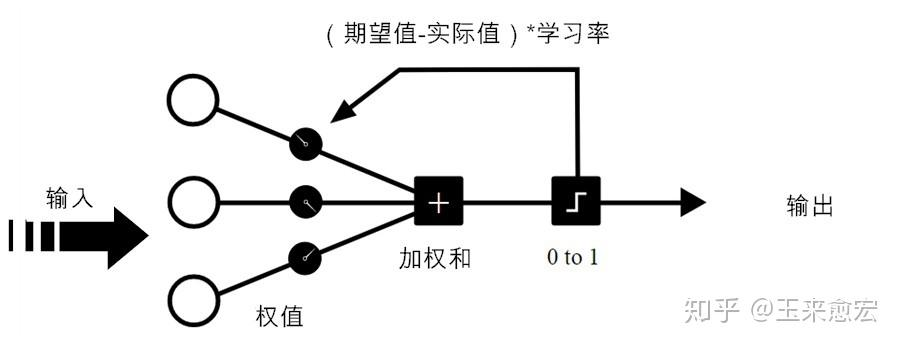
\includegraphics[width=0.8\textwidth]{figs/罗森布拉特提出的感知机模型.jpg}
\caption{罗森布拉特提出的感知机模型}
\label{罗森布拉特提出的感知机模型}
\end{figure}

学着，学着，这部感知机就能“感知”出最佳的连接权值。然后，对于一个全新的图片，在没有任何人工干预的情况下，它能“独立”判定出图片标识为左还是为右。这个过程，不就与小孩子的学习差不多吗？儿童成长的第一阶段（从出生到2岁，相当于婴儿期）就是感知阶段。此阶段的儿童主要靠感觉和动作探索周围的世界，逐渐形成物体永存性观念，慢慢就有了自己对事物的独立判断。

在发明感知机之后，时年30岁的罗森布拉特，意气风发，迫不及待地召开新闻发布会，畅谈自己研究成果的美好未来，吸引了众多媒体的极大关注。其中，就包括大名鼎鼎的《纽约时报》（The New York Times）。

纽约时报记者对科技非常敏感，也被罗森布拉特发明的感知机模型所折服。1958年7月8日，《纽约时报》在头版报道了罗森布拉特的研究成果，《纽约时报》记者对感知机的先进性赞不绝口，报道说，
{\bf“ 这是一个能够行走、拥有视觉、能够写作、能自我复制，且有自我意识的电子计算机的雏形”。}

要知道，文章刊发时，距离标志着人工智能学科诞生的达特茅斯（Dartmouth）会议（1956年夏季）的召开，仅仅过去两年。纽约时报对人工智能的憧憬，放到六十多年后的今天，仍然毫不过时。文章当时还非常乐观地估计，

“再花上10万美元，一年以后，上述构想就能实现可期。那时，感知机将能够识别出人，并能叫出他们的名字，而且还能把人们演讲的内容即时地翻译成另一种语言或记录下来。”
可能是嫌《纽约时报》的报道不够深入，在那篇头版文章发表几天后，1958年7月13日，罗森布拉特亲自上阵，撰文于《纽约时报》，文章的题目是“Electronic 'Brain' Teaches Itself（能自学的电脑）”。 当下，我们常爱用“电脑”称呼“计算机”，如果追溯起来，或许这个词最早就是罗森布拉特杜撰出来的。

在那篇亲笔题写的文章里，罗森布拉特正式把自己设计的算法，取名为“感知机”。同时，他不忘“吹捧”自己研究成果的历史地位：

不依赖于人类的训练和控制，感知机有望成为能感知、会识别、可确认周边环境的第一个非生命机理。
六十年过去了，有个叫凯文•凯利（Kevin Kelly）的科技预言家，写了一本很有影响力的书，叫《必然》[2]。在书中，凯文•凯利说，

未来科技将有12大进化趋势，其中第2大趋势就是“知化（Cognifying）”。
那什么是“知化”呢？所谓的“知化”，就是让一个事物具备认知能力。

凯文•凯利认为，人工智能的本质就是“知化”，即硬件问题软件化。现在，细想一下，罗森布拉特提出的感知机的构想，大概就是一种“知化”的体现，在当时的确是属于最先进的人工智能，因为他的畅想放在六十年后的今天，仍不过时。

 1957年，Frank Rosenblatt 基于 M-P 模型提出了感知机（Perceptron），这是第一个实现了参数自动更新的神经元模型。  
 
 所谓的感知机，其实就是一个由两层神经元构成的网络结构，它在输入层接收外界的输入，通过激活函数（含阈值）的变换，把信号传送至输出层，因此它也称之为“阈值逻辑单元（threshold logic unit）”。

感知机后来成为许多神经网络的基础，但它的理论基础依然建立于皮茨等人提出来的“M-P神经元模型”。

感知机虽然简单，但已初具神经网络的必备要素。在前面我们也提到，所有“有监督”的学习，在某种程度上，都是分类（classification）学习算法。而感知机就是有监督的学习，因此它也是一种分类算法。

感知机的目标是通过训练学习输入和输出之间的映射关系。它采用简单的更新规则优化权重：
 $$ w_i \leftarrow w_i+ \eta (y-\hat{y}) x_i$$
 其中，~$y$为真实输出，~$\hat y$为模型预测值，~$\eta$为学习率，~$x_i$为输入。 
 
 通过逐步调整权重，感知机能够在给定的训练集上实现正确分类。然而，由于感知机只能解决线性可分问题，其局限性也催生了多层神经网络的研究。
 
 
 举例
 
 下面我们就列举一个分区分“西瓜和香蕉”的经典案例，来看看感知机是如何工作的[3]。根据第6章的介绍，感知机模型的形式化描述可用公式（7-1）呈现
 \begin{equation}\label{feature}
 y = w_1x_1+w_2x_2+\cdots + w_nx_n -\theta
 \end{equation}
为了简单起见，我们假设西瓜和香蕉都仅有两个特征（feature）：形状和颜色，其它特征暂不考虑。这两个特征都是基于视觉刺激而最易得到的。

假设特征~$x_1$代表输入颜色，特征~$x_2$代表形状，权重~$w_1$和~$w_2$默认值暂且都设为1，为了进一步简化，我们把阈值 （亦有教程称之为偏置——bias）设置为0 。为了标识方便，我们将感知机输出数字化，如果输出为“1”，则代表判定为“西瓜”，而输出为“0”，代表判定为“香蕉”。当然了，如果有更多类别的物品，我们就用更多的数字来标记即可，示意图~\ref{感知机学习算法示意图}所示。
\begin{figure}[htbp]
\centering
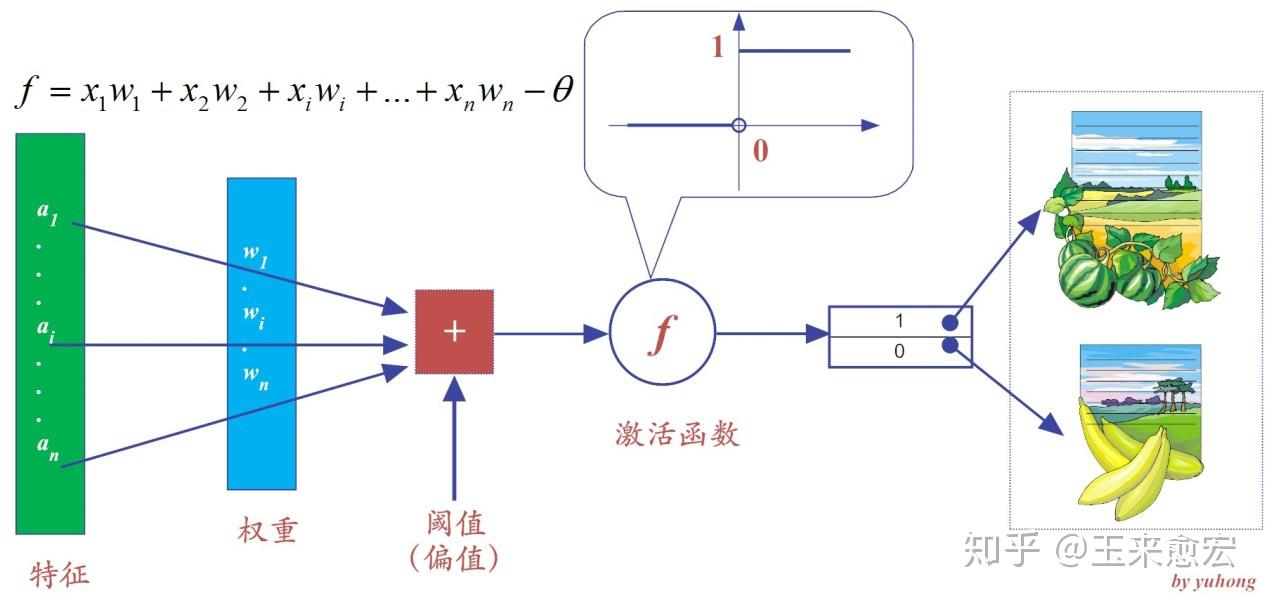
\includegraphics[width=0.8\textwidth]{figs/感知机学习算法示意图.jpg}
\caption{感知机学习算法示意图}
\label{感知机学习算法示意图}
\end{figure}
 
 感知机的激活函数
 
为了方便机器计算，我们对颜色和形状这两个特征，给予不同的值，以示区别。比如，颜色这个特征为绿色时，$x_1$取值为1，而当颜色为黄色时，$x_1$取值为-1；类似地，如果形状这个特征为圆形，$x_2$取值为1，反之，形状为弯曲状时，$x_2$取值为-1，如表\ref{西瓜与香蕉的特征值表}所示。

\begin{table}[htbp]
\centering
\begin{tabular}{|c|c|c|c|
}
\hline
{\bf 品类} & {\bf  颜色($x_1$) } & {\bf 形状($x_2$)}  \\
\hline
{\bf 西瓜} &  1 (绿色)  &  1 (圆形)   \\
\hline
{\bf 香蕉}  &  -1 (黄色) & -1 (弯形)  \\
\hline
\end{tabular}
\caption{西瓜与香蕉的特征值表}
\label{西瓜与香蕉的特征值表}
\end{table}

这样一来，可以很容易依据公式（\ref{feature}）描述的感知机模型，对于西瓜、香蕉做鉴定（即输出函数f的值），其结果分别如图\ref{感知机的输出}(a)所示：

\begin{figure}[htbp]
\centering
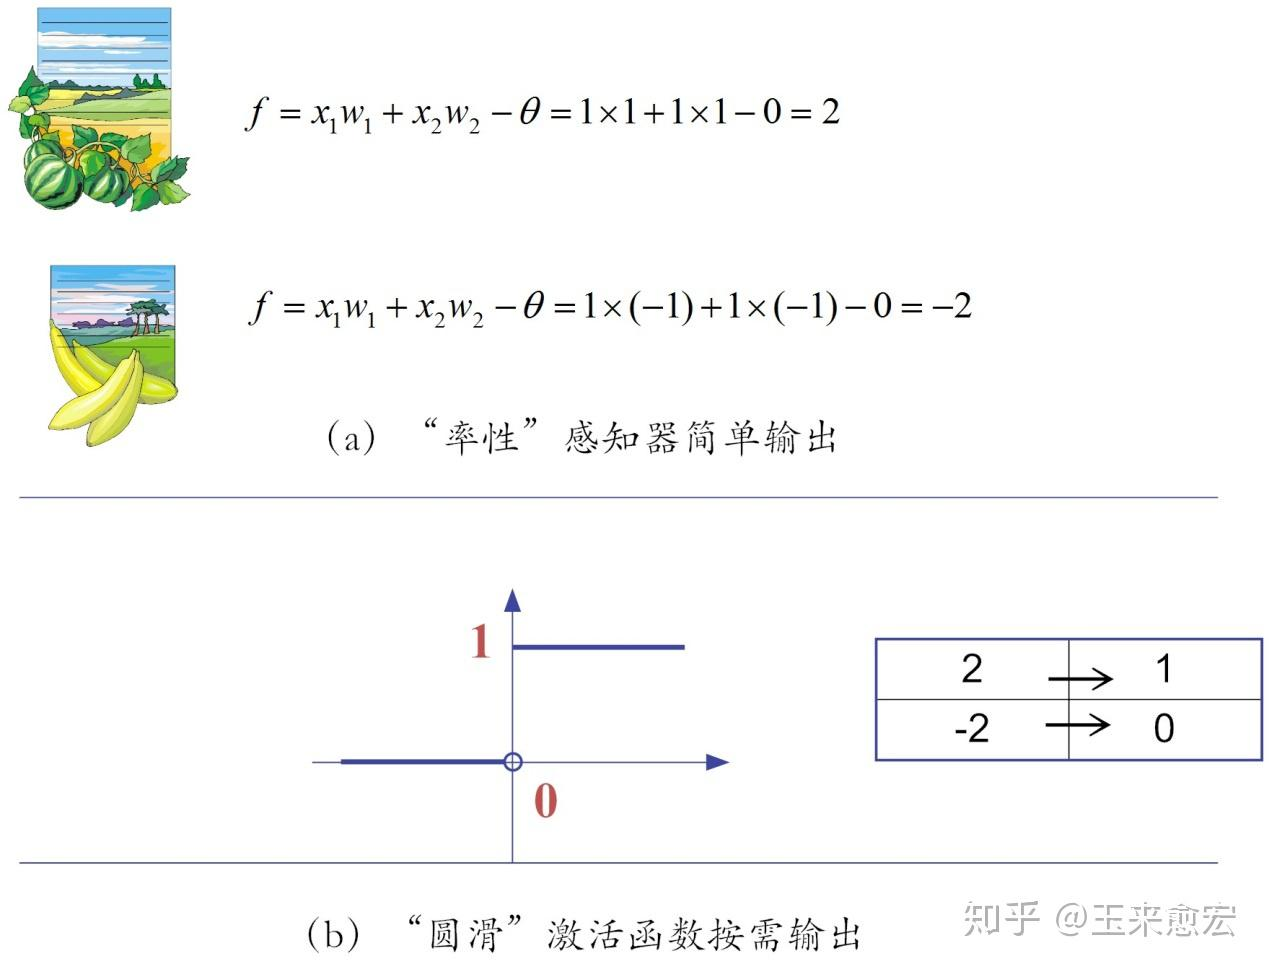
\includegraphics[width=0.8\textwidth]{figs/感知机的输出.jpg}
\caption{感知机的输出}
\label{感知机的输出}
\end{figure}
 
 
从图\ref{感知机的输出}(a)所示的输出可以看到，对西瓜的判定输出结果是2，而香蕉的为-2。而我们先前预定的规则是：函数输出为1，则判定为西瓜，输出为0，则判定为香蕉，那么如何将2或-2这样的分类结果，变换成预期的分类表达呢，这个时候，就需要激活函数上场了！

激活函数的作用，在本质上，就是变换映射空间。

标准的前馈型神经网络层（输入层除外），它的实现的变换可以分为线性组合和非线性激活两步。传统普遍使用的激活函数有sigmoid函数和tanh函数，较新的有ReLU（详见 ）。

这里的激活函数，我们使用了最原始、最为简单的阶跃函数（step function），它可以模拟神经元的激活或抑制。在阶跃函数中，输出规则非常简单：当~$ x \ge 0$时， 输出为1，否则输出0。通过激活函数的“润滑”之后，结果就变成我们想要的样子（如图\ref{感知机的输出}(b)所示）。就这样，我们就搞定了西瓜和香蕉的判定。

这里需要说明的是，对象的不同特征（比如水果的颜色或形状等），只要用不同数值区分表示开来即可，具体用什么样的值，其实并无大碍。

但你或许会疑惑，这里的阈值（threshold） 和两个连接权值~$w_1$和~$w_2$，为啥就这么巧分别就是0、1、1呢？如果取其它数值，会有不同的判定结果吗？

这是个好问题。事实上，我们并不能一开始就知道这几个参数的取值，而是一点点地“折腾”（Try-Error）出来的，而这里的“折腾”其实就是感知机的学习过程！

% 对单神经元模型，给出训练方法：根据输出~$y$与期望输出~$y^*$之间的误差，调整权重~$w_i$  来完成学习。
 
 模型：
 $$
 g({\bf x},{\bf w}) =\left\{ \begin{array}{cl} 
 +1 & \mbox{当 }{\bf w}^T{\bf x}>0 \\
  -1 & \mbox{当 }{\bf w}^T {\bf x}<0
  \end{array}
 \right. = {\rm sign}({\bf w}\cdot {\bf x} +b)
 $$

损失函数 ~$L({\bf w};{\bf x},y) = {\rm max}(0, -y {\bf w}^T {\bf x}). $

优化：随机梯度下降


感知机参数学习的更新过程

https://zhuanlan.zhihu.com/p/40396252
感知机是如何工作的？

中国有句古话：
“知错能改，善莫大焉。”
说的就是，犯了错误而能改正，没有比这更好的事了。

\begin{figure}[htbp]
\centering
\begin{subfigure}{0.9\linewidth}
\centering
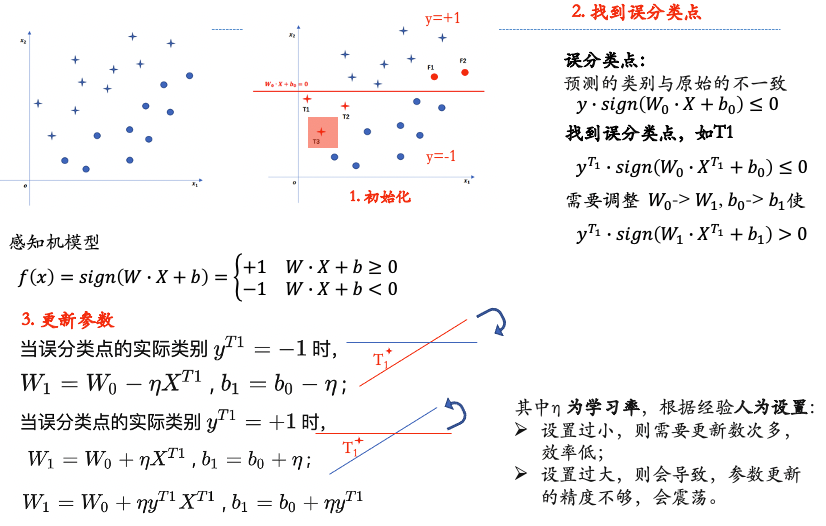
\includegraphics[width=1\linewidth]{figs/参数更新1.png}
\caption{参数更新过程一}
\label{参数更新1}
\end{subfigure}

\begin{subfigure}{0.9\linewidth}
\centering
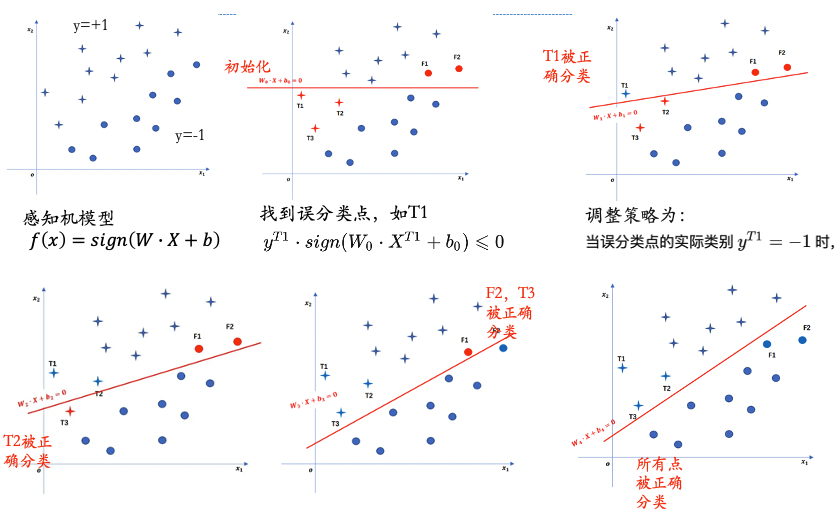
\includegraphics[width=1\textwidth]{figs/参数更新2.png}
\caption{生物神经元与人工神经元}
\label{参数更新2}
\end{subfigure}
\caption{参数更新过程一}
\label{感知机参数学习的更新过程}
\end{figure}


我们期望输出的正确判定是：$y=1$，而现在实际输出的值$=0$，也就是说，实际输出有误。这个时候，就需要纠偏。而纠偏，就需要利用公式（7-2）所示的学习规则。于是，我们需要计算出误差。

是二者的“落差”。在后面，读者可以看到，这个“落差”就是整个网络中权值和阈值的调整动力。很显然，如果为0，即没有误差可言，那么新、旧权值和阈值都是一样的，网络就稳定可用了！


在这个示例里，仅仅经过一轮“试错法”，我们就搞定了参数的训练，但你可别高兴太早，谁叫这是一个“Hello World”版本的神经网络呢！

事实上，在有监督的学习规则中，我们需要根据输出与期望值的“落差”，经过多轮重试，反复调整神经网络的权值，直至这个“落差”收敛到能够忍受的范围之内，训练才告结束。


感知机的几何意义
下面我们来分析一下感知机的几何意义。由感知机的功能函数定义可知，它是由两个函数复合而成：内部为神经元的输出汇集函数，外部为激活函数，将汇集函数的输出，作为激活函数的输入。如果识别对象x有n个特征，内部函数就是如下公式所示的输入汇集。
\begin{figure}[htbp]
\centering
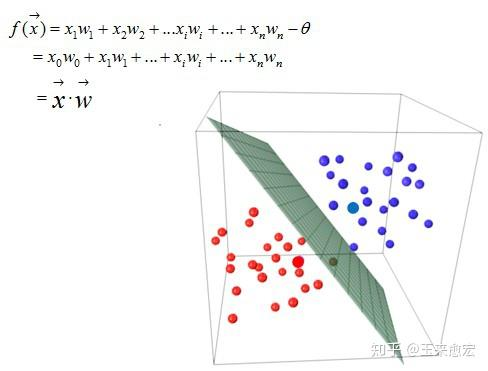
\includegraphics[width=1\textwidth]{figs/感知机的超平面.jpg}
\caption{感知机的超平面}
\label{感知机的超平面}
\end{figure}

若令其等于零，即，该方程可视为一个在$n$维空间的超平面$P$。那么感知机以向量的模式写出来就是：（如图7-6所示），这里，“”表示输入向量$x$和权值向量$w$的内积。

这样一来的话，对于超平面一侧的实例，它表示点落在超平面的正半空间，此时激活函数，即感知机输出为1（判定为正类），而对于超平面的另外一侧实例，表示点落在超平面的负半空间，此时激活函数，即感知机输出为0（判定为负类）。

于是，感知机可看做一个由超平面划分的空间位置的识别器。

当特征~$n$为两三个维度时，人们尚可利用它的几何空间来直观解释这个分类器，但当$n$更大时，人们很难再用它的几何意义来研究神经网络。


感知机的超平面

应用1：图像分类
\begin{figure}[htbp]
\centering
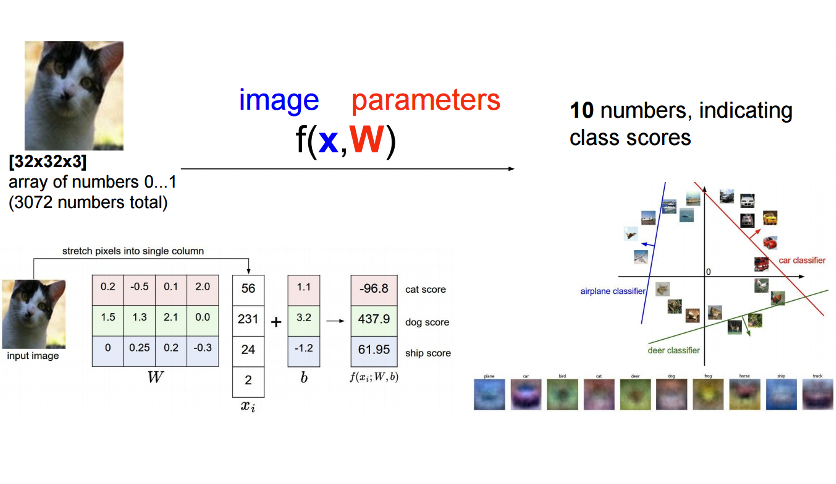
\includegraphics[width=1\textwidth]{figs/图像分类.png}
\caption{图像分类}
\label{图像分类}
\end{figure}

应用2：文本分类
\begin{figure}[htbp]
\centering
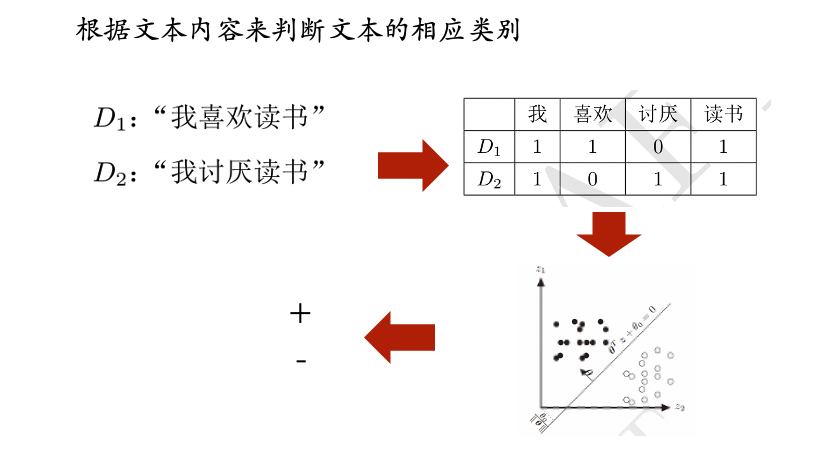
\includegraphics[width=1\textwidth]{figs/文本分类.png}
\caption{文本分类}
\label{文本分类}
\end{figure}

{\bf 无所不能的感知机模型？}

“无论什么问题，只要明确了输入和输出之间的关系，都可能通过学习得以解决。”


致命打击：1969年Marvin Minsky 和 Papert指出，感知机连一个简单的XOR问题都无法完成。

可以解决：二分类且线性可分问题

不能解决异或 (同或)问题

 
导致了研究的低潮。

\subsection{从简单到深度：多层感知机的崛起}
感知机的局限性在于它无法解决非线性问题，比如判断一个图案是否包含交叉的线条。为了突破这个瓶颈，科学家们提出了多层感知机（MLP）。它的基本思路是：在输入层和输出层之间加入隐藏层，每层通过非线性激活函数进一步提取数据的复杂特征。

多层感知机的提出让神经网络从简单走向复杂，也让深度学习成为可能。特别是在计算能力和数据规模迅速增长的今天，深度学习已经在语音识别、图像分类和自然语言处理等领域大放异彩。

\begin{figure}[htbp]
\centering
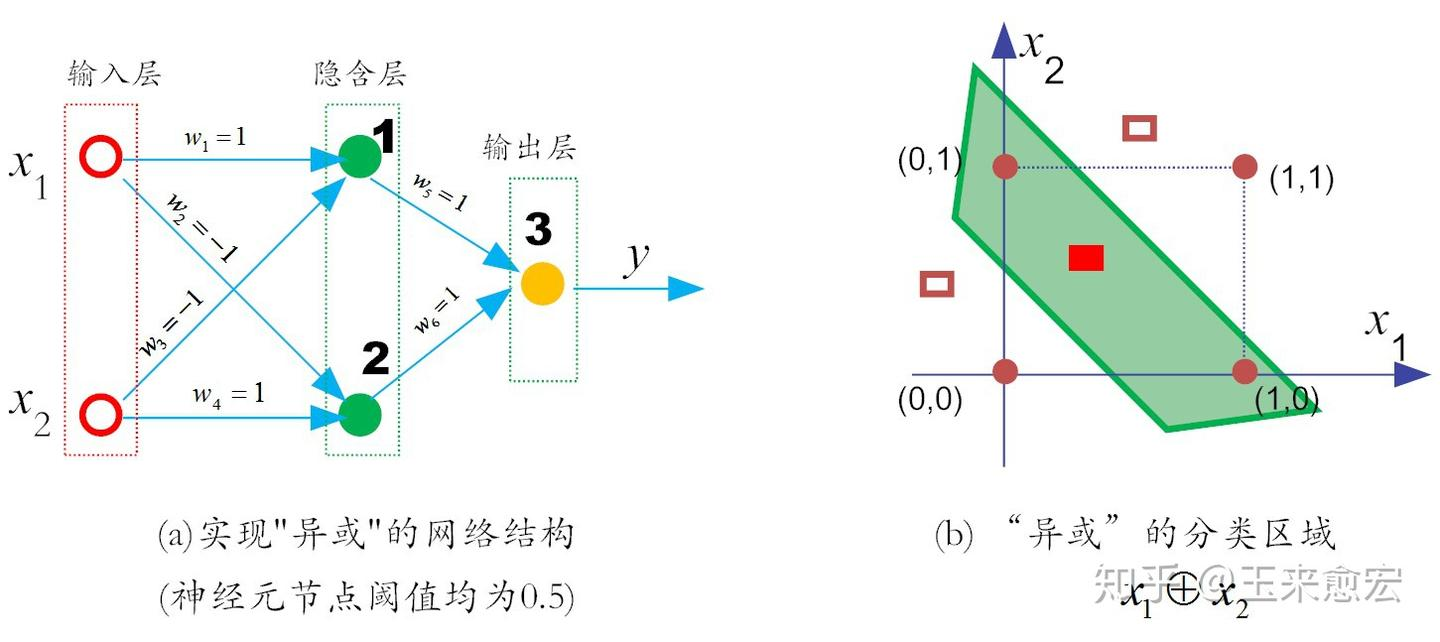
\includegraphics[width=1\textwidth]{figs/可解决“异或”问题的两层感知机.jpg}
\caption{可解决“异或”问题的两层感知机}
\label{可解决“异或”问题的两层感知机}
\end{figure}



如前文所述，想解决“异或”问题，就需要让网络复杂起来。这是因为，复杂的网络，表征能力就比较强[1]。按照这个思路，可以在输入层和输出层之间，添加一层神经元，将其称之为隐含层（hidden layer，亦有文献简称为“隐藏层”、“隐层”，后文不再区分这三个称谓）。这样一来，隐含层和输出层中的神经元都拥有激活函数。假设各个神经元的阈值均为0.5，权值如图\ref{可解决“异或”问题的两层感知机}所示，就实现了“异或”功能（在后续的章节中，我们会给出多层感知机解决“异或”问题的Python实战案例）。

解决异或问题的方案
下面我们来详述这个实现流程。假设在如图8-1-(a)所示的神经元（即实心圆），其激活函数依然是阶跃函数（即sgn函数），它的输出规则非常简单：当~$x\ge 0$ 时，~$f(x)$输出为1，否则输出0。

那么，对于和相同（假设均为1）时，神经元对隐层节点1和2的权重分别为~$w_1=1$和~$w_2=-1$，神经元对隐层节点1和2的权重分别为$w_3=-1$和$w_4=1$。于是，对于在隐层的神经元1来说，其输出可以表述为：
$$
f_1 ={\rm sgn}(x_1w_1 +x_2 w_2 -\theta) ={\rm sgn}(1\times 1 +1\times (-1)-0.5) ={\rm sgn}(-0.5) =0
$$
类似地，对于在隐层的神经元2有,
$$
f_2 ={\rm sgn}(x_1w_3 +x_2 w_4 -\theta) ={\rm sgn}(1\times (-1) +1\times 1-0.5) ={\rm sgn}(-0.5) =0
$$
然后，对于输出层的输出神经元3而言，这时~$f_1$和~$f_2$是它的输入，于是有：
$$
y=f_3 ={\rm sgn}(f_1w_5 +f_2 w_6 -\theta) ={\rm sgn}(0\times 1 +0\times (-1)-0.5) ={\rm sgn}(-0.5) =0
$$
也就是说，~$x_1$和~$x_2$同为1时，输出为0，满足了“异或”的功能。读者朋友也可以尝试推导一下，~$x_1$和~$x_2$同为0时的情况，这个简单的两层感知机输出为0，也就是说满足“异或”的功能。

那么对于~$x_1$和~$x_2$不相同（假设~$x_1=1$时，~$x_2=0$）时，对于在隐含层的神经元1有：
$$
f_1 ={\rm sgn}(x_1w_1 +x_2 w_2 -\theta) ={\rm sgn}(1\times 1 +0\times (-1)-0.5) ={\rm sgn}(0.5) =1
$$
类似地，对于在隐层的神经元2有,
$$
f_2 ={\rm sgn}(x_1w_3 +x_2 w_4 -\theta) ={\rm sgn}(1\times (-1) +0\times 1-0.5) ={\rm sgn}(-1.5) =0
$$
然后，对于输出层的输出神经元3而言，这时~$f_1$和~$f_2$是它的输入，于是有：
$$
y=f_3 ={\rm sgn}(f_1w_5 +f_2 w_6 -\theta) ={\rm sgn}(1\times 1 +0\times 0-0.5) ={\rm sgn}(0.5) =1
$$

https://zhuanlan.zhihu.com/p/42041080

不失一般性，由于~$x_1$和~$x_2$的地位是可以互换的。也就是说，当~$x_1$和~$x_2$取值不同时，感知机输出为1。因此，从上面分析可知，如图8-1所示的两层感知机，可以实现“异或”功能。在这里，网络中的权值和阈值是我们事先给定的，而实际上，它们是需要神经网络自己通过反复地“试错”学习而来，而且能够完成“异或”功能的网络权重也不是唯一的。


1958年，弗兰克·罗森布拉特（Frank Rosenblatt）提出“感知机”（Perceptron）的概念。

1965年，A. G.伊瓦赫年科（Alexey Grigorevich Ivakhnenko）就提出了多层人工神经网络的设想。回想一下，1971 年 7 月 11 日，罗森布拉特在自己的生日那天，离奇溺水身亡。有人猜测，罗是被明斯基“怼”死的。而如果有人提前注意到几年前伊瓦赫年科的工作，用多层感知机就能解决异或问题，就不会让明斯基如此发飙，而让罗如此难堪。罗之死，多少有点冤啊。

而这种基于多层神经网络的机器学习模型，后来被人们称为“深度学习”。简单来说，所谓深度学习，就是包括很多隐含层的神经网络学习。

这里的“深”即意味着“层深”（’Deep’ means many hidden layers），“网络深深深几许”呢？至少要大于3吧，多则不限，可以成百甚至上千。

所以，你看到了吧，如果追根溯源的话，伊瓦赫年科才是“深度学习”之父，而不是现在的“深度学习”大牛杰弗里•辛顿（Geoffrey Hinton），但鉴于辛顿的杰出贡献——是他让“深度学习”重见天日、大放异彩。因此，称呼辛顿为“深度学习教父（Godfather of deep learning）”，似乎也更为合适。

更需要我们玩味的是，在多层神经网络概念提出4年之后的1969年，明斯基才写出来他的那本“毒苹果”之作《感知机》。也就是说，多层神经网络在提出之后，并没有受到应有的重视。

直到1975年（此时，距离伊瓦赫年科提出多层神经网络概念已达10年之久了），感知机的“异或难题”才被理论界彻底解决。由此，见微知著可以看到，科学技术的发展，从来都不是线性地一蹴而就，而是呈现螺旋上升的！

我们现在学习这个“异或”解决方案，可能仅需要数分钟，但也真是“书上一分钟，书后十年功”！

\subsection{ 多层感知机：包含1个或多个隐层的前馈神经网络}
1974年，Geoffrey Hinton第一次挽回联结学派的败局，提出“多则不同”，把多个感知机连接成一个分层网络，从而可处理非线性可分问题。
 (Multilayer Perceptron, MLP) 
 
\begin{figure}[htbp]
\centering
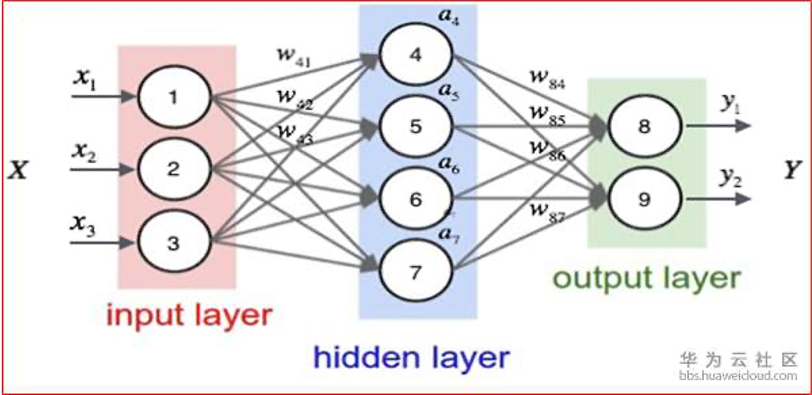
\includegraphics[width=1\textwidth]{figs/MLP.png}
\caption{多层感知机网络}
\label{MLP}
\end{figure}

\section{深度学习的数学灵魂：万能近似定理}

深度学习并不仅仅是“多加几层网络”这么简单。它的成功依赖于一套强大的数学框架，这套框架赋予了神经网络非凡的学习能力。

机器学习在本质上，就是找好一个好用的函数。而人工神经网络最牛的地方可能就在于，它可以在理论上证明：“一个包含足够多隐层神经元的多层前馈网络，能以任意精度逼近任意预定的连续函数~\ref{HORNIK1989359}”。

这个定理也被称之为通用近似定理（Universal Approximation Theorem）。这里的“Universal”，也有人将其翻译成“万能的”，由此可以看出来，这个定理的能量有多大。
\begin{figure}[htbp]
\centering
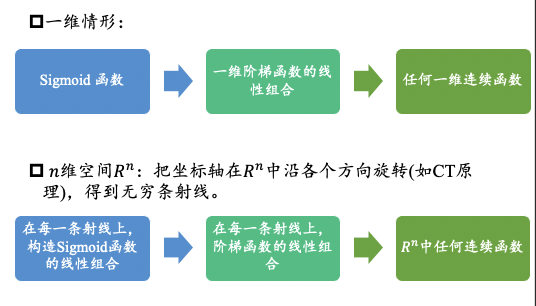
\includegraphics[width=1\textwidth]{figs/万能近似定理.png}
\caption{万能近似定理}
\label{万能近似定理}
\end{figure}

万能逼近定理指出：一个单隐层神经网络只要神经元足够多，就能逼近任何连续函数。这听起来很神奇，但也说明了神经网络的强大表达能力。

“万能近似定理”告诉我们，不管函数 
 在形式上有多复杂，我们总能确保找到一个神经网络，对任何可能的输入x，以任意高的精度近似输出值为f(x)（如图2-4所示）。即使函数有多个输入和输出，即 
 ，通用近似定理的结论也是成立的。换句话说，神经网络在理论上可近似解决任何问题，这就厉害了！有关神经网络可以计算任何函数的可视化证明，感兴趣的读者可以参阅Michael Nielsen的博客文章[2]。

使用这个定理时，我们需要注意如下两点：

（1）定理说的是，可以设计一个神经网络尽可能好地去“近似”某个特定函数，而不是说“准确”计算这个函数。我们通过增加隐层神经元的个数来提升近似的精度。

（2）被近似的函数，必须是连续函数。如果函数是非连续的，也就是说有极陡跳跃的函数，神经网络就“爱莫能助”了。

即使函数是连续的，有关神经网络能不能解决所有问题，也是有争议的。原因很简单，就如同那句玩笑话“理想很丰满，现实很骨感”说得那样，通用近似定理在理论上是一回事，而在实际操作又是另外一回事。

比如，深度学习新秀、生成对抗网络（GAN）发明者 Ian Goodfellow就曾发表意见说，“仅含有一层的前馈网络，的确足以有效地表示任何函数，但是，这样的网络结构可能会格外庞大，进而无法正确地学习和泛化:

"A feedforward network with a single layer is sufficient to represent any function, but the layer may be infeasibly large and may fail to learn and generalize correctly。”
Goodfellow的言外之意是说，“广而浅薄”的神经网络在理论上是万能的，但在实践中却不是那么回事。因此，网络往“深”的方向去做，才是正途。（这个议题，回头我们再深入探讨）

事实上，1989年“通用近似定理”就被提出了，到2006年深度学习开始厚积而薄发，这期间神经网络并没有因为这个理论而得到蓬勃发展。因此，从某种程度上，验证了Goodfellow的判断。

\subsection{ 激活函数}

激活函数是深度学习的灵魂，它为神经网络注入了非线性，让模型能够捕捉复杂的特征。比如，ReLU函数的简单性和效率，使其成为深度学习的“主力军”。



激活函数是神经网络的关键组件，用于引入非线性能力，使网络能够表达复杂的模式。常见的激活函数包括：

Sigmoid 函数：用于将输出限制在 $[0, 1]$ 范围。
ReLU 函数：高效且常用，解决了梯度消失问题。
Tanh 函数：扩展了 Sigmoid 的输出范围至 $[-1, 1]$。


{\bf 非线性表达需要激活函数}

任何线性函数的线性组合仍然是线性的。
没有激活函数，神经网络就是线性函数，不能解决任何非线性问题。




{\bf  通用近似定理(universal approximation theorem) (Hornik et al., 1989; Cybenko, 1989) }

对于具有线性输出层和至少一个使用 “挤压”性质的激活函数的隐藏层组成的前馈神经网络，只要其隐藏层神经元的数量足够，可以以任意精度近似任一个定义在实数空间中的有界闭集函数。

一个两层的神经网络可以模拟任何函数。



神经网络能逼近任何函数：分段是关键。任何函数，可以用“分段”线性函数来逼近

激活函数，让神经网络具备“分段”表达能力。

\begin{figure}[htbp]
\centering
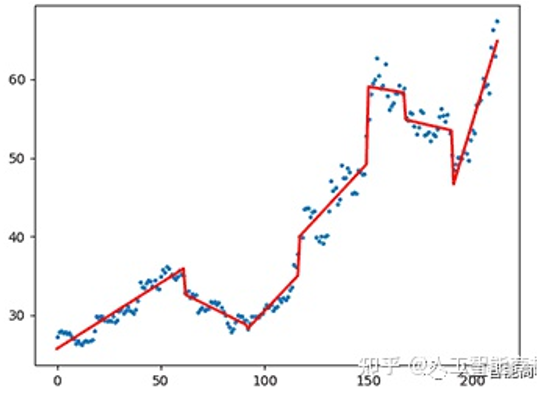
\includegraphics[width=0.69\textwidth]{figs/分段线性逼近.png}
\caption{分段线性函数的逼近}
\label{分段线性逼近}
\end{figure}


{\bf 激活函数的分段功能} 

激活函数为神经网络提供“分段”能力的来源。
激活函数 activation =“打开”+ “截断”能力
Relu激活函数
	输入~$𝑥<0$ 时，输出~$𝑦=0$ ，实现截断(关闭)功能
	输入~$𝑥>0$ 时，输出~$𝑦=𝑥$，实现导通(打开)功能。
激活函数的“分段”能力，把线性函数，组合成折线函数（分段函数），可以让神经网络逼近任何函数。

{\bf 神经网络近似任意函数的示例}

最简单的神经网络：最后一层是Sigmoid函数：
一个线性函数经过Sigmoid扭曲为一条“S型”曲线。

只要有足够多的分段函数，并仔细调整它们的权重，就能近似任意的函数。

思想类似于傅里叶级数定理：复杂周期运动 = 多个周期运动之和
      非周期运动 = 无穷个周期运动之和



%\begin{figure}[htbp]
%\centering
%begin{subfigure}{0.6\linewidth}
%\centering
%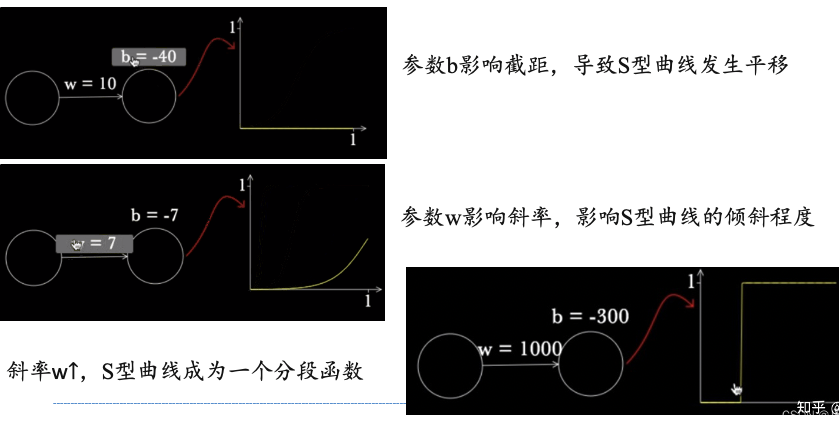
\includegraphics[width=1\linewidth]{figs/神经网络近似任意函数.png}
%\caption{神经网络近似任意函数}
%\label{神经网络近似任意函数}
%\end{subfigure}
%
%begin{subfigure}{0.6\linewidth}
%\centering
%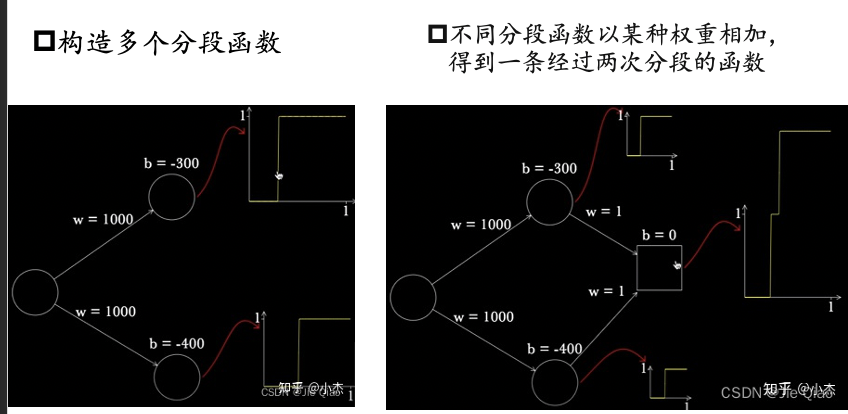
\includegraphics[width=1\linewidth]{figs/神经网络近似任意函数2.png}
%\caption{神经网络近似任意函数2}
%\label{神经网络近似任意函数2}
%\end{subfigure}
%\caption{神经网络近似任意函数}
%\label{神经网络近似任意函数}
%\end{figure}



{\bf 万能近似原理的一维与~$n$维情形}


\begin{figure}[htbp]
\centering
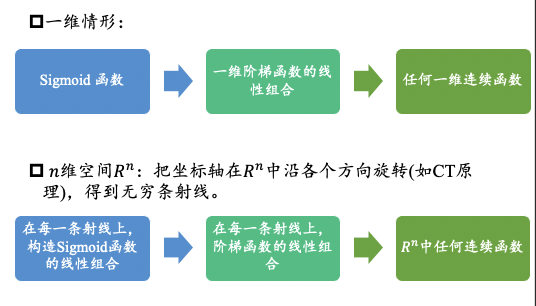
\includegraphics[width=0.69\textwidth]{figs/万能近似定理.png}
\caption{万能近似定理}
\label{万能近似定理}
\end{figure}


截断能力最强的是阶跃函数和ReLu函数，其它激活函数：“软化”版（折线变曲或变缓）
梯度下降法需要求解相邻层的梯度，这要求网络中处处可导，故激活函数需满足可导性。
M-P模型中使用step函数作为激活函数，只能输出0或1，不连续不可导。
后续提出可导函数sigmoid作为激活函数---梯度饱和问题
发展出ReLU函数及其变形激活函数


\begin{figure}[htbp]
\centering
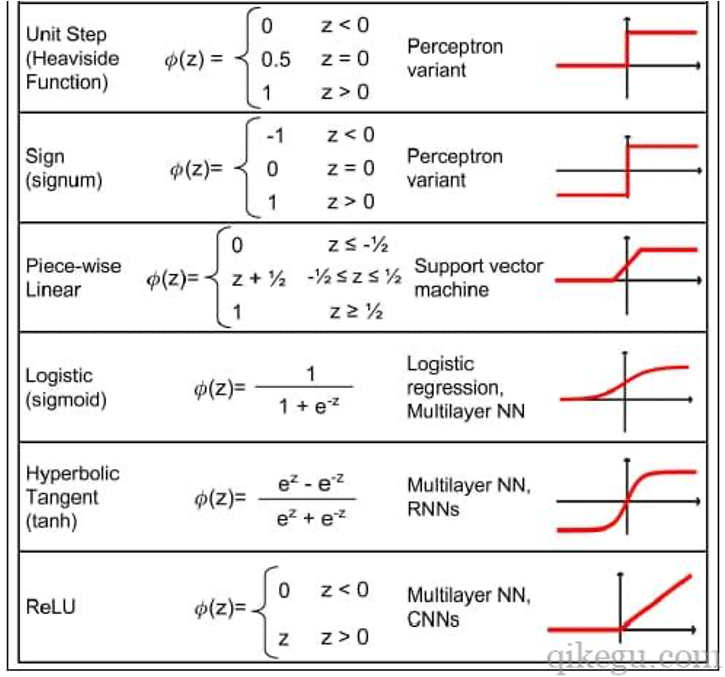
\includegraphics[width=0.69\textwidth]{figs/激活函数.png}
\caption{激活函数}
\label{激活函数}
\end{figure}

{\bf  Unit Step Function (Heaviside Function)}

{\bf  Unit Step Function (Heaviside Function)}

{\bf  Piece-wise Linear }


{\bf  Logisitic (sigmoid)}

劣势：
输入趋近无穷时会导致梯度趋近于零：引起梯度弥散
所有输出值均为正值，不以零为中心：影响神经网络收敛速度

如何改进---Tanh函数：
以零为中心的对称函数，收敛速度快
仍然无法解决梯度弥散问题

梦魇： “梯度消失”现象严重。
梯度指数衰减后，在反向传播时，底层基本上接受不到有效的训练信号。
如，幅度为1的信号，在反向传播梯度时，每传递一层，梯度衰减为原来的0.25。




新函数的应用：
在DNN的发展中，ReLU、maxout等传输函数代替了 Sigmoid，解决了梯度消失问题。


融合使用的试验：e.g. Sigmoid系的Acrtan函数和ReLU函数的融合


{\bf Hyperbolic Tangent(tanh)  }

{\bf  ReLU 函数 (Rectified Linear Unit，ReLU)}

ReLU函数
分散、稀疏，避免了Sigmoid系函数的饱和情况
有利于梯度下降和反向传播算法，避免梯度爆炸和梯度消失
小于零的部分均为零：硬饱和性，均值偏移

1. 计算速度快
2. 生物上的原因
3. 解决梯度下降问题


\begin{figure}[htbp]
\centering
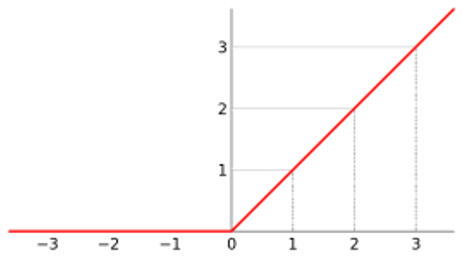
\includegraphics[width=0.69\textwidth]{figs/ReLU.png}
\caption{ReLU}
\label{ReLU}
\end{figure}


\begin{figure}[htbp]
\centering
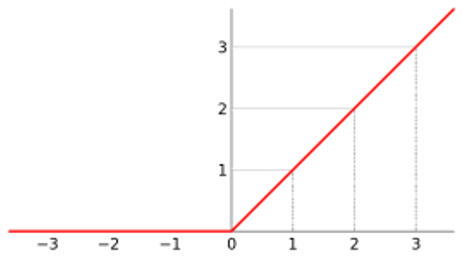
\includegraphics[width=0.69\textwidth]{figs/ReLU.png}
\caption{ReLU}
\label{ReLU}
\end{figure}


%\begin{figure}[htbp]
%\centering
%begin{subfigure}{0.6\linewidth}
%\centering
%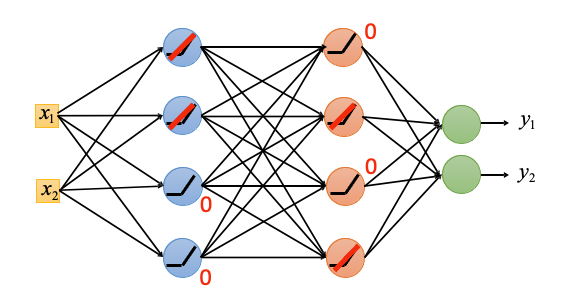
\includegraphics[width=1\linewidth]{figs/ReLU-network.png}
%%\caption{}
%\label{ReLU-network}
%\end{subfigure}

%begin{subfigure}{0.6\linewidth}
%\centering
%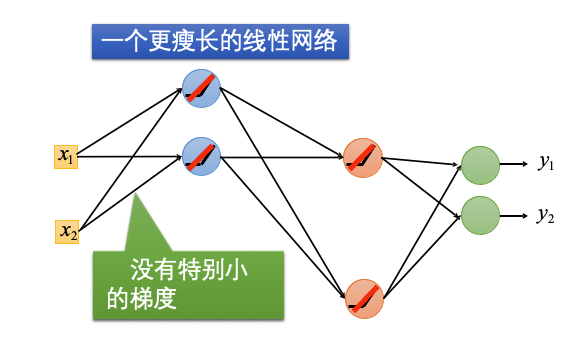
\includegraphics[width=1\linewidth]{figs/ReLU-network2.png}
%%\caption{}
%\label{ReLU-network2}
%\end{subfigure}
%\caption{神经网络近似任意函数}
%\label{神经网络近似任意函数}
%\end{figure}
%
%\begin{figure}[htbp]
%\centering
%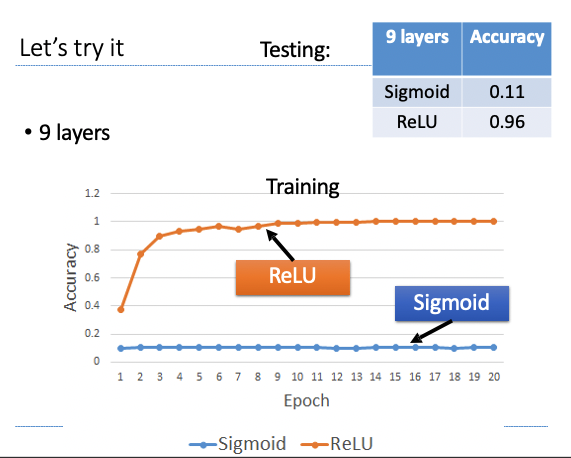
\includegraphics[width=0.69\textwidth]{figs/experiement.png}
%\caption{ReLU 函数与Sigmoid 函数对比}
%\label{experiement}
%\end{figure}
%

{\bf  Arctan}

Arctan函数
基本性质类似Sigmoid函数
输出范围在 (- π / 2 , π / 2 )
比Sigmoid函数和Tanh函数图像更为和缓，饱和区间较大
导数趋于零的速度更慢，导数计算更加昂贵，但缓解了梯度消失问题

\begin{figure}[htbp]
\centering
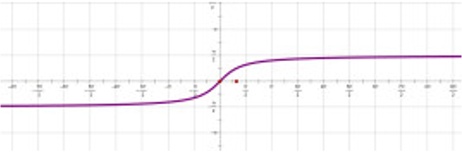
\includegraphics[width=0.69\textwidth]{figs/arctan.png}
\caption{arctan}
\label{arctan}
\end{figure}


{\bf AcrReLU函数}

~$x>0$的部分采用ReLU函数
~$x\le0$的部分采用Acrtan函数


实验效果：
初始的累积误差小，具有较快的收敛速度。
有效缓解梯度消失问题
缓解ReLU负轴部分的硬饱和性
AUC值更大，泛化性能更优
但计算消耗较昂贵，时间较久
\begin{figure}[htbp]
\centering
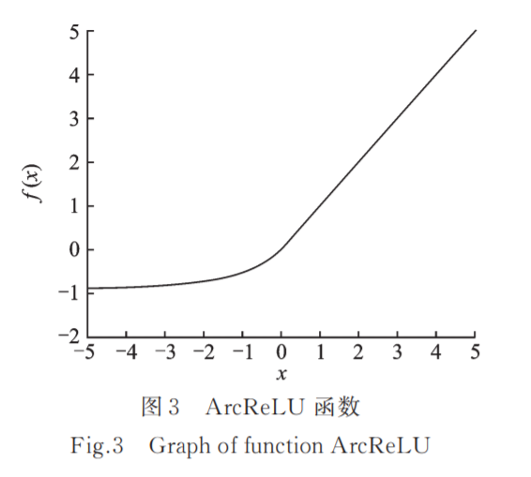
\includegraphics[width=0.69\textwidth]{figs/arcReLU.png}
\caption{arcReLU}
\label{arcReLU}
\end{figure}


\subsection*{ “没有免费的午餐”定理}
没有免费的午餐定理（No Free Lunch Theorem）指出，没有一种万能的学习算法能在所有任务上都优于其他算法。这意味着深度学习虽然强大，但也需要在具体任务中找到合适的模型和优化方法。

\subsection{ 人工神经网络：从简单到深度}

人工神经网络（Artificial Neural Networks，ANNs）是对感知机的扩展，通过引入多层结构解决了非线性问题。

多层网络的优势
多层神经网络由输入层、隐藏层和输出层组成。隐藏层的引入使得网络能够提取数据的多层次特征，克服了单层网络无法处理非线性问题的局限性。

深度学习的革命
随着计算能力的提升和反向传播算法的提出，深度神经网络（Deep Neural Networks，DNNs）成为可能。多层结构使得神经网络在复杂任务中表现卓越，从而推动了深度学习的快速发展。


人工神经网络=大量的神经元的有向连接

1.神经元的激活规则：神经元的输入到输出之间的(非线性)映射关系
2.网络的拓扑结构：不同神经元之间的连接关系
3.学习算法：通过训练数据来学习神经网络的参数

\begin{figure}[htbp]
\centering
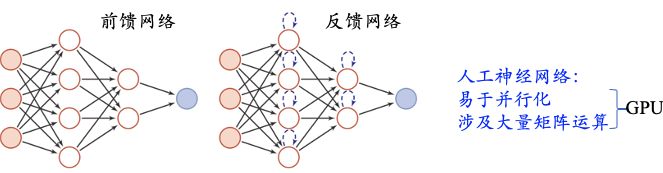
\includegraphics[width=1\textwidth]{figs/ANN2.png}
\caption{}
\label{ANN2}
\end{figure}




\section{深度学习的方法论}

再议“end-to-end”（端到端）

在深度学习中，经常有“end-to-end（端到端）”学习的提法，与之相对应的传统机器学习是“Divide and Conquer（分而治之）”。这些都是什么意思呢？

“end-to-end”（端到端）说的是，输入的是原始数据（始端），然后输出的直接就是最终目标（末端），中间过程不可知，也难以知。比如说，基于深度学习的图像识别系统，输入端是图片的像素数据，而输出端直接就是或猫或狗的判定。这个端到端就是：像素判定。

再比如，“end-to-end”的自动驾驶系统，输入的是前置摄像头的视频信号（其实也就是像素），而输出的直接就是控制车辆行驶指令（方向盘的旋转角度）。这个端到端就是：像素指令。


就此，有人批评深度学习就是一个黑箱（Black Box）系统，其性能很好，却不知道为何而好，也就是说，缺乏解释性。其实，这是由于深度学习所处的知识象限决定的。深度学习，在本质上，属于可统计不可推理的范畴。“可统计”是很容易理解的，就是说，对于同类数据，它具有一定的统计规律，这是一切统计学习的基本假设。那“不可推理”又是什么概念？其实就是“剪不断、理还乱”的非线性状态了。


从哲学上讲，这种非线性状态，是具备了整体性的“复杂系统”，属于复杂性科学范畴。复杂性科学认为，构成复杂系统的各个要素，自成体系，但阡陌纵横，其内部结构难以分割。简单来说，对于复杂系统，1+1≠2，也就是说，一个简单系统，加上另外一个简单系统，其效果绝不是两个系统的简单累加效应，而可能是大于部分之和。因此，我们必须从整体上认识这样的复杂系统。于是，在认知上，就有了从一个系统或状态（end）直接整体变迁到另外一个系统或状态（end）的形态。这就是深度学习背后的方法论。

与之对应的是“Divide and Conquer（分而治之）”，其理念正好相反，在哲学它属于“还原主义（Reductionism，或称还原论）”。在这种方法论中，有一种“追本溯源”的蕴意包含其内，即一个系统（或理论）无论多复杂，都可以分解、分解、再分解，直到能够还原到逻辑原点。

在意象上，还原主义就是“1+1=2”，也就是说，一个复杂的系统，都可以由简单的系统简单叠加而成（可以理解为线性系统），如果各个简单系统的问题解决了，那么整体的问题也就得以解决。比如说，很多的经典力学问题，不论形式有多复杂，通过不断的分解和还原，最后都可以通过牛顿的三大定律得以解决。

从传统的“还原论”出发，单纯的线性组合思维，势必就会导致人工智能系统的设计，功能过于简单。如果我们希望模拟的是一个“类人”的复杂系统（即人工智能系统），自然就无法有效达到目的，具体说来，有如下两个方面的原因：

（1）这个世界（特别是有关人的世界）本身是个纷纭复杂的系统，问题之间互相影响，形成复杂的网络，这样的复杂系统，很难利用一个或几个简单的公式、定理来描述和界定。
（2）在很多场景下，受现有测量和认知工具的局限，很多问题在认识上根本就不具有完备性。因此，难以从一个“残缺”的认知中，提取适用于全局视角的公式和定理。
对于这个复杂的世界，直接抓住它的规律并准确描述它，是非常困难的。在一个复杂系统中，由于非线性因素的存在，任何局部信息都不可能代表全局。大数据时代有个典型的特征就是，“不是随机样本，而是全体数据（n=all）”，而“全体数据”和复杂性科学中“整体性”，在一定程度上，是有逻辑对应关系的。

\section{深度神经网络的结构}

深度学习的三大核心组成部分：

神经网络结构：从简单的全连接网络到卷积神经网络（CNN）、循环神经网络（RNN）等。
训练过程：通过梯度下降法和反向传播算法调整网络参数。
损失函数：定义优化目标，例如交叉熵损失用于分类，均方误差用于回归。


针对前馈神经网络，输入层和输出层设计比较直观。针对神经网络，我们拆开想想What和How的问题：

1）神经：即神经元，什么是神经元（What）？
2）网络：即连接权重和偏置，它们是怎么连接的（How）？
对于计算机而言，它能计算的就是一些数值。而数值的意义是人赋予的。法国著名数学家、哲学家笛卡尔曾在它的著作《谈谈方法》提到：“我想，所以我是”。文雅一点的翻译就是“我思故我在”。套用在神经元的认知上，也是恰当的。这世上本没有什么人工神经元，你（人）认为它是，它就是了。也就是说，数值的逻辑意义，是人给的。

比如说，假如我们尝试判断一张手写数字图片上面是否写着数字“2”。很自然地，我们可以把图片的每一个像素的灰度值，作为网络的输入。从笛卡尔“我思故我在”角度来看，在输入层，每个像素都是一个数值（如果是彩色图，则是3通道的数组），而把包容这个数值的容器视作一个神经元。

 输入层神经元个数的设计
如果图片的维度是16×16，那么我们输入层神经元就可以设计为256个（也就是说，输入层是一个包括256个灰度值的向量），每个神经元接受的输入值，就是归一化处理之后的灰度值。0代表白色像素，黑色像素像素代表1，灰度像素的值介于0到1之间。也就是说，输入向量的维度（像素个数）要和输入层神经元个数相同。

\begin{figure}[htbp]
\centering
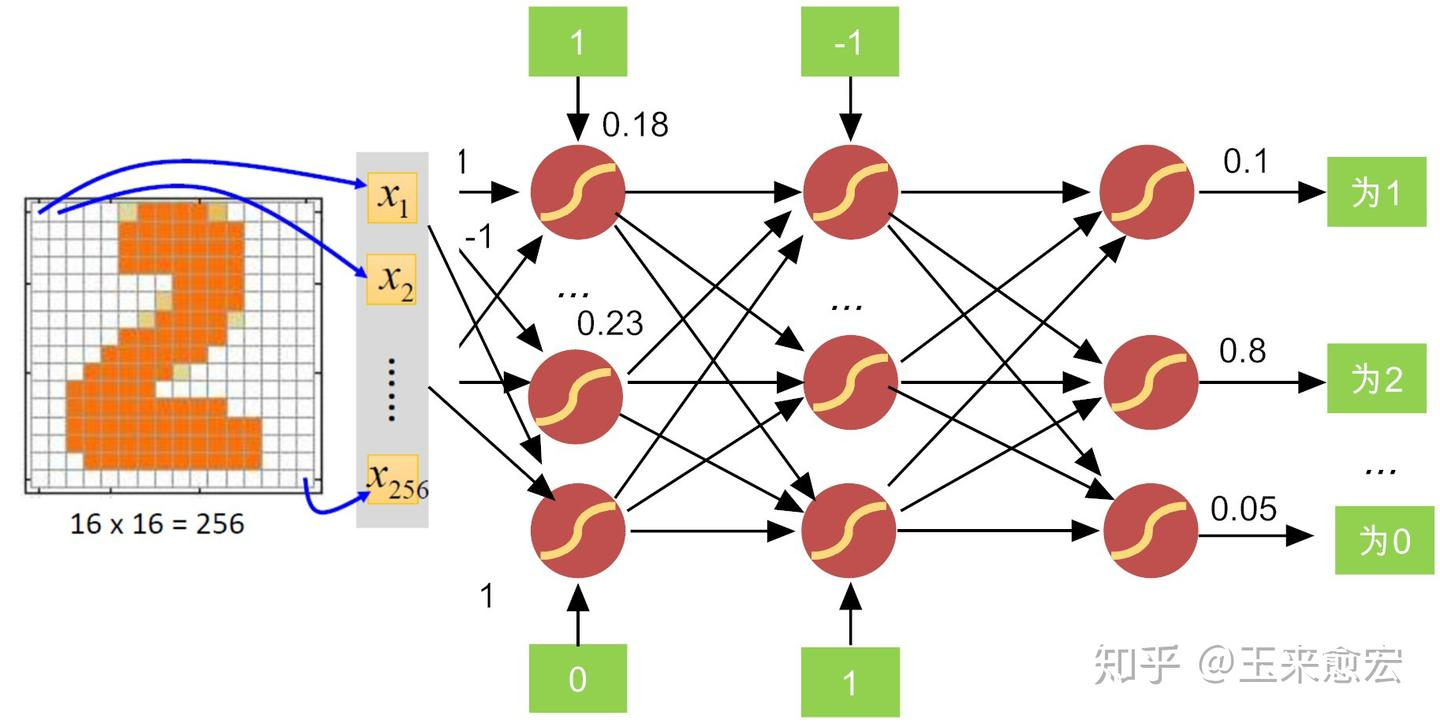
\includegraphics[width=0.69\textwidth]{figs/前馈神经网络的输出.jpg}
\caption{前馈神经网络的输出}
\label{前馈神经网络的输出}
\end{figure}

输入层神经元个数的设计
而对输出层而言，它的神经元个数和输入神经元的个数，是没有对应关系的，而是和待分事物类别有一定的相关性。

比如说，对于图\ref{前馈神经网络的输出}所示的案例，我们的任务是识别手写数字，而数字有0~9共10类。所以，如果在输出层采用Softmax回归函数，它的输出神经元数量仅为10个，分别对应是数字“0~9”的分类概率。

最终的分类结果，择其大者而判之。比如说，如果判定为“2”的概率（比如说80\%），远远大于其他数字，那么整个神经网络的最终判定，就是手写图片中的数字是“2”，而非其它数字。

9.4 隐含层神经元个数的设计
相比于神经网络输入与输出层设计的明了直观，前馈神经网络的隐含层设计，可就没有那么简单了。说好听点，它是一门艺术，依赖于“工匠”的打磨。说不好听点，它就是一个体力活，需要不断地折腾“试错”。

我们可以把隐含层暂定为一个黑箱，它负责输入和输出之间的非线性映射变化，具体功能有点“说不清、道不明”（这是神经网络的理论短板所在）。隐含层的层数不固定，每层的神经元个数也不固定，它们都属于“超参数”，是人们根据实际情况不断调整选取的。

前面我们讨论了什么是神经元。下面我们再讨论一下神经元之间是如何连接的。事实上，它同样是人赋予意义的数值参数。我们把神经元与神经元之间的影响程度叫作为权值（weight）。权重的大小就是连接的强弱。它“告诉”下一层相邻神经元更应该关注那些像素图案。

除了连接权值，神经元内部还有一个施加于自身的特殊权值，叫偏置（bias）。有了偏置，它能辅助神经元是否更容易被激活。也就是说，它决定神经元的连接加权和得有多大，才能让激发变得有意义。

神经网络结构的设计目的在于，让神经网络以“更佳”的性能来学习。而这里的所谓“学习”，就是找到合适的权重和偏置，让损失函数的值达到最小。



\subsection{卷积神经网络（CNN）}
CNN 专为处理图像数据设计，通过卷积操作提取局部特征。其特点包括局部感受野、共享权重和池化操作。CNN 在图像分类、目标检测和图像生成等领域取得了显著成果。


卷积神经网络（Convolutional Neural Networks, CNN）是专为处理具有网格结构数据（如图像和时间序列）而设计的神经网络。其核心在于通过卷积操作提取数据的局部特征，从而有效降低高维数据的计算复杂度，并捕获关键的模式和结构。

核心数学思维
CNN 的核心数学基础是卷积操作，它通过滑动滤波器在数据上执行局部运算来提取特征。

卷积操作：提取局部特征
卷积操作本质上是一种数学运算，用于两个函数之间的相关性计算。在图像处理中，卷积通常可以表示为以下公式：
$$𝑆(𝑖,𝑗)=\sum_{𝑚} \sum_𝑛 𝑋(𝑖+𝑚,𝑗+𝑛)
\cdot 𝐾(𝑚,𝑛)$$
其中，~$X(i,j) $是输入图像的像素值，~$K(m,n)$ 是卷积核（滤波器），也称为权重矩阵。~$S(i,j)$ 是卷积操作后的输出特征图。

卷积核通过与图像的局部区域进行点积运算，输出一个新的特征值。这种局部化的计算方式具有以下优势：

参数共享：相同的卷积核在图像的不同区域滑动，极大地减少了参数数量。
稀疏连接：卷积核只与输入数据的局部区域相连接，从而降低了计算复杂度。

\subsubsection*{卷积神经网络的核心组成部分}
1. 卷积层（Convolution Layer）：

通过多个卷积核提取输入数据的局部特征。每个卷积核可以学习到特定的模式（如图像中的边缘、纹理）。
输出特征图的大小可以通过以下公式计算：
$$
Output Size=
\frac{Input Size -Kernel Size+2\cdot Padding}{Stride}+1$$

2. 激活函数

常用 ReLU（Rectified Linear Unit）作为非线性激活函数，定义为：
$$
f(x)=max(0,x)$$

ReLU 引入了非线性能力，使网络能够拟合复杂的模式。

3. 池化层（Pooling Layer）：

池化层用于对特征图进行下采样，减少数据维度并保留关键特征。常见的池化操作包括最大池化（Max Pooling）和平均池化（Average Pooling）。

最大池化公式：
$$P(i,j)=max(X_{m,n}) ,m,n\in Kernel Region$$

全连接层（Fully Connected Layer）：

将卷积层和池化层提取的特征展平，并通过全连接层进行分类或回归。

深层卷积网络的特性

1. 层级特征表示：

CNN 通过多层卷积逐步提取数据的高级特征。例如：
第一层卷积：检测边缘等低级特征。
中间层卷积：提取纹理、形状等中级特征。
高层卷积：捕获语义信息（如图像中的物体类别）。

权值共享和参数共享：

卷积核在整个输入数据上共享参数，从而减少了模型的训练参数，降低了过拟合的风险。

局部连接：

CNN 的每个神经元只连接到输入数据的局部区域，而不是与所有像素相连。这种局部连接的机制有效提升了计算效率。


数学直观：卷积如何看世界
可以将卷积核视为“特征检测器”。在图像处理中，不同的卷积核会响应不同的模式：

检测边缘的卷积核可能对亮暗变化敏感。
检测形状的卷积核会捕捉到特定的几何结构。

当卷积层堆叠在一起时，CNN 能够逐步从简单的边缘特征构建出复杂的全局模式。

CNN 的典型应用

图像分类：
CNN 在 ImageNet 图像分类挑战赛中多次刷新记录，成为计算机视觉的主流工具。

目标检测：
Faster R-CNN 和 YOLO 等模型利用卷积网络定位和分类图像中的目标。

图像生成：
GAN（生成对抗网络）利用卷积层生成高质量的图像。

卷积神经网络的核心数学思维，使其能够在保持计算效率的同时，捕获高维数据中的深层特征。这种能力让 CNN 成为处理图像和视频数据的首选工具，并推动了深度学习在多个领域的突破性进展。


\subsection{循环神经网络}

RNN 适用于处理序列数据，通过隐藏状态捕获时间依赖信息。然而，传统 RNN 存在梯度消失问题，改进的 LSTM 和 GRU 模型显著提升了其性能。RNN 被广泛用于语音识别、机器翻译和文本生成任务。


\section{小结}

\begin{figure}[htbp]
\centering

\includegraphics[width=1\textwidth]{figs/认知.png}
\caption{认知世界：我们对自身了解多少？}
\label{neuron}
\end{figure}

科学的本质之一是揭示“我们是怎么知道的”，深度学习的发展为这一追问提供了技术上的回答。从对生物大脑的模拟到人工神经网络的建立，深度学习不仅是一种技术，也是一种科学方法论的进步。

通过模仿生物神经网络，构建多层神经网络，深度学习实现了从简单到复杂、从线性到非线性的飞跃。它的每一步进化，都让我们离构建真正的智能机器更近了一步。


\newpage